%%
%% IMWUT Manuscript: Proactive Affective Agent
%%
\documentclass[screen,review,anonymous]{acmart}

\AtBeginDocument{%
  \providecommand\BibTeX{{%
    Bib\TeX}}}

%% Journal information
\acmJournal{IMWUT}
\acmVolume{0}
\acmNumber{0}
\acmArticle{0}
\acmYear{2026}
\acmMonth{9}

%% Packages
\usepackage{booktabs}
\usepackage{multirow}
\usepackage{subcaption}
\usepackage{xcolor}
\usepackage{soul}
\usepackage{enumitem}
\usepackage{tikz}
\usetikzlibrary{positioning, arrows.meta, fit, decorations.pathreplacing, calc}
\usepackage{pgfplots}
\pgfplotsset{compat=1.18}

%% Custom commands
\newcommand{\sys}{Proactive Affective Agent}
\newcommand{\sysshort}{PULSE}
\newcommand{\todo}[1]{\textcolor{red}{\textbf{[TODO: #1]}}}
\newcommand{\ba}{\text{BA}}
\newcommand{\maemetric}{\text{MAE}}
\newcommand{\erdesire}{ER\textsubscript{desire}}
\newcommand{\intavail}{INT\textsubscript{avail}}

\begin{document}

%% Title
\title{PULSE: Agentic Sensing for Proactive Intervention in Cancer Survivorship}

%% Authors (anonymized for review)
\author{Anonymous Author(s)}
\affiliation{%
  \institution{Anonymous Institution}
}

%% Abstract
\begin{abstract}
Proactive mental health support for cancer survivors requires anticipating intervention needs from passive behavioral signals---yet the people who most need help are least likely to self-report. \sysshort{} addresses this challenge with LLM agents that \emph{autonomously investigate} smartphone sensing data (8 modalities at hourly resolution) through purpose-built tools for sensor querying, personalized baseline comparison, and population-level calibration via retrieval-augmented generation. Rather than receiving pre-formatted feature summaries, agents plan their own investigation strategy---deciding which modalities to probe and how deeply---mirroring hypothesis-driven clinical reasoning. We evaluate a 2$\times$2 factorial design (structured vs.\ agentic reasoning $\times$ sensing-only vs.\ multimodal) on 50 cancer survivors from the BUCS longitudinal study (${\sim}$3,900 entries per condition). When diary text is available, the best agentic multimodal agent (Auto-Multi+) achieves balanced accuracy of 0.751 for emotion regulation desire, 0.722 for negative affect state, and 0.733 for positive affect state (mean BA = 0.661 across all targets vs.\ 0.629 for the best supervised baseline). Critically, even without any self-report, sensing-only agentic agents predict intervention availability at BA = 0.706---demonstrating viable proactive prediction from passive data alone. These findings suggest that LLM agents equipped to selectively query and reason over behavioral sensor streams can outperform both fixed analytical pipelines and traditional machine learning, advancing the feasibility of proactive just-in-time adaptive interventions.
\end{abstract}

%% CCS Concepts
\begin{CCSXML}
<ccs2012>
   <concept>
       <concept_id>10003120.10003121.10003129</concept_id>
       <concept_desc>Human-centered computing~Ubiquitous and mobile computing systems and tools</concept_desc>
       <concept_significance>500</concept_significance>
   </concept>
   <concept>
       <concept_id>10010147.10010178.10010187</concept_id>
       <concept_desc>Computing methodologies~Natural language processing</concept_desc>
       <concept_significance>300</concept_significance>
   </concept>
</ccs2012>
\end{CCSXML}

\ccsdesc[500]{Human-centered computing~Ubiquitous and mobile computing systems and tools}
\ccsdesc[300]{Computing methodologies~Natural language processing}

\keywords{Just-in-time adaptive interventions, passive sensing, large language models, affective computing, cancer survivorship, agentic AI}

%% Teaser figure — appears between title and abstract in acmart
\begin{teaserfigure}
  \centering
  \includegraphics[width=\textwidth]{figures/fig_teaser.pdf}
  \caption{\sysshort{} addresses ambiguity in ultra-brief diary entries by integrating passive behavioral sensing with agentic investigation. A diary entry alone admits multiple interpretations (left); always-on smartphone sensors reveal behavioral context (center); the \sysshort{} agent autonomously queries sensor data through purpose-built tools to disambiguate affect and predict intervention need (right).}
  \Description{A three-panel figure showing the PULSE pipeline: (1) an ambiguous diary entry with three possible interpretations, (2) passive smartphone sensors including GPS, motion, screen, and diary, and (3) the PULSE agent using tools to produce binary state predictions for positive affect, negative affect, regulation desire, and intervention availability.}
  \label{fig:teaser}
\end{teaserfigure}

\maketitle

%% ================================================================
%%  1. INTRODUCTION
%% ================================================================
\section{Introduction}

Cancer survivors face persistent psychosocial challenges that extend far beyond treatment completion~\cite{stanton2012cancer_survivorship}. Fear of recurrence, chronic fatigue, anxiety, and depression affect up to 40\% of long-term survivors, yet the majority lack access to continuous psychological support~\cite{hagan2022cancer_fear}. Just-in-time adaptive interventions (JITAIs)---systems that deliver support at moments of need based on real-time contextual data---hold considerable promise for addressing this gap~\cite{nahum2018jitai}. The core premise is compelling: rather than waiting for scheduled therapy sessions, an intelligent system could detect emerging distress and offer coping strategies precisely when a survivor is both \emph{in need} and \emph{available} to engage.

Realizing this vision, however, confronts a fundamental paradox. Current JITAI systems overwhelmingly rely on \emph{active self-report}---ecological momentary assessments (EMAs), daily diaries, or mood check-ins---to sense users' emotional states~\cite{shiffman2008ema}. Yet the individuals who most urgently need intervention are precisely those who are least likely to complete self-reports: elevated stress reduces motivation to engage with survey prompts, while low energy and social withdrawal diminish the likelihood of timely responses~\cite{mishra2021receptivity}. A system that can only act when told how the user feels is fundamentally \emph{reactive}---it cannot help those who have stopped talking.

Passive smartphone sensing offers a path toward \emph{proactive} intervention. Modern smartphones continuously collect rich behavioral signals---movement patterns, location traces, screen usage, typing behavior, app engagement---that correlate with psychological states~\cite{saeb2015phenotyping, wang2014studentlife, wang2018sensing}. However, translating these noisy, heterogeneous sensor streams into actionable emotional state predictions has proven difficult. Traditional machine learning approaches treat sensing features as fixed tabular inputs, applying random forests or gradient boosted trees to daily aggregate statistics~\cite{xu2023globem}. These methods capture coarse statistical associations but struggle with the contextual interpretation that distinguishes a ``stayed home all day because of illness'' from a ``stayed home all day because it's a holiday''---the same behavioral pattern with radically different affective implications.

Recent advances in large language models (LLMs) suggest a fundamentally different approach. LLMs can interpret behavioral data described in natural language, generating contextually grounded hypotheses that statistical models cannot express. Prior work has shown that LLMs achieve competitive performance on emotion recognition from text~\cite{yang2024llm_mental, amin2023llm_ema} and can interpret wearable sensor data when presented as natural language descriptions~\cite{kim2024health_llm, xu2024penetrative_ai}. CALLM~\cite{wang2026callm} demonstrated that LLMs can predict emotional states from cancer survivors' diary text with balanced accuracy exceeding traditional NLP approaches---but CALLM remains fundamentally reactive, requiring users to write diary entries, and cannot operate when self-report is absent.

A key limitation of prior LLM-based approaches is that they receive pre-formatted data summaries---the model reasons about what it is given, but cannot decide what to look at. Recent work on agentic AI has shown that giving LLMs autonomous access to external tools enables multi-step investigation~\cite{yao2023react, schick2024toolformer}, and health-focused systems like PHIA~\cite{merrill2025phia} and GLOSS~\cite{min2025gloss} have applied agentic tool-use to wearable data analysis and sensemaking. However, no prior work has used agentic investigation for \emph{prospective prediction} of affective states in a clinical population, nor systematically compared agentic vs.\ structured approaches through controlled experimentation.

In this paper, we ask two questions: \emph{(1) can LLM agents predict intervention opportunities from passive sensing data, and (2) does giving them the autonomy to investigate sensor data---deciding which modalities to query, how far back to look, and which anomalies to pursue---improve prediction over fixed analytical pipelines?}

We introduce the \emph{\sys{}} (\sysshort{}), an LLM-based framework for predicting emotional states and intervention opportunities in cancer survivors. \sysshort{} treats each prediction as a \emph{behavioral investigation}: rather than receiving a fixed feature vector, the agent autonomously queries a sensing database through tool-use (function calling), planning its own investigation strategy across multiple reasoning turns. We define this \emph{autonomously-agentic} approach as one where the LLM controls the investigation loop---selecting tools, interpreting results, and deciding whether to query further---in contrast to \emph{structured-agentic} approaches where the reasoning pipeline is fixed. This mirrors how a clinical behavioral scientist might reason: starting with a broad overview, forming hypotheses, and drilling into specific signals that seem informative.

Our core contribution is a systematic evaluation of this agentic paradigm through a 2$\times$2 factorial design:

\begin{itemize}[nosep]
    \item \textbf{Structured vs.\ Agentic reasoning}: Should the LLM follow a fixed analytical pipeline, or autonomously decide how to investigate the data?
    \item \textbf{Sensing-only vs.\ Multimodal data}: Can passive sensing alone support prediction, or is diary text essential?
\end{itemize}

\noindent This yields four agent variants (Struct-Sense, Auto-Sense, Struct-Multi, and Auto-Multi), evaluated alongside a diary-only baseline (CALLM) and traditional ML/DL baselines, on data from the BUCS cancer survivorship study~\cite{wang2026callm}---a longitudinal dataset of 418 participants with 15,984 EMA entries and 8 passive sensing modalities at hourly resolution. We additionally evaluate filtered variants (Auto-Sense+, Auto-Multi+) that receive pre-processed behavioral narratives with redundant data removed.

We focus on predicting \emph{intervention opportunity}, which we define as the conjunction of two constructs:
\begin{enumerate}[nosep]
    \item \textbf{Emotion regulation desire} (\erdesire{}): Does the user want emotional support right now?
    \item \textbf{Intervention availability} (\intavail{}): Is the user able to engage with an intervention right now?
\end{enumerate}

\noindent An effective JITAI must detect both: a willing but unavailable user cannot engage, while an available but uninterested user will not. Alongside intervention opportunity, we evaluate prediction of positive and negative affect states (PANAS scales~\cite{watson1988panas}), which inform the \emph{type} of support to offer.

Our evaluation across 50 cancer survivors (${\sim}$3,900 EMA entries per condition) reveals:

\begin{enumerate}[nosep]
    \item \textbf{Agentic investigation outperforms structured pipelines} for binary state detection (paired Wilcoxon $p < 10^{-10}$ on per-user mean BA). Giving LLM agents autonomous control over their sensing queries yields significant improvements over fixed analytical pipelines in both sensing-only and multimodal conditions.

    \item \textbf{Multimodal data (sensing + diary) outperforms either modality alone}, with the best agentic multimodal agent achieving mean BA of 0.661 across all binary targets vs.\ 0.629 for the best supervised baseline.

    \item \textbf{Sensing-only agents enable viable proactive prediction}. Even without diary text, agentic sensing-only agents predict intervention availability at BA = 0.706, demonstrating that passive behavioral data alone can support intervention timing---the core requirement for proactive systems.
\end{enumerate}

\noindent To our knowledge, this is the first work to apply agentic LLM investigation to \emph{prospective affective state prediction} in a clinical population with a controlled factorial comparison. While prior systems (GLOSS~\cite{min2025gloss}, PHIA~\cite{merrill2025phia}) apply agentic tool-use to health data analysis, they target retrospective sensemaking rather than real-time prediction. Our results suggest that combining LLM reasoning with passive smartphone sensing advances the feasibility of proactive mental health support. We note that our evaluation is retrospective---predictions are made on historical data with temporal boundaries enforced---and that translation to real-time deployment remains future work.

%% ================================================================
%%  2. RELATED WORK
%% ================================================================
\section{Related Work}

\subsection{Passive Sensing for Mental Health}

Smartphone-based passive sensing has emerged as a scalable approach to mental health monitoring~\cite{torous2016smartphone_psychiatry, jacobson2019digital_phenotyping}. Pioneering work by Saeb et al.~\cite{saeb2015phenotyping} demonstrated significant correlations between GPS-derived mobility features and depression severity. The StudentLife study~\cite{wang2014studentlife} established that passively collected sensor data---including sleep, physical activity, and social interaction patterns---correlate with mental health outcomes, academic performance, and behavioral changes in college students. Subsequent work expanded these findings to clinical populations: Wang et al.~\cite{wang2018sensing} tracked depression dynamics via mobile sensing, Rashid et al.~\cite{rashid2020predicting} predicted social anxiety from sparse mobile data, and Canzian and Musolesi~\cite{canzian2015trajectories} detected depressive episodes from GPS trajectories. CrossCheck~\cite{ben_zeev2015crosscheck} demonstrated continuous monitoring of schizophrenia symptoms, while Gr{\"u}nerbl et al.~\cite{gruenerbl2015phone_depression} recognized bipolar states from smartphone data. Doryab et al.~\cite{doryab2019modeling_behavior} identified behavioral phenotypes of loneliness and social isolation, and Wahle et al.~\cite{wahle2016mobile_sensing} showed the feasibility of mobile sensing for depression support in the wild.

The GLOBEM benchmark~\cite{xu2023globem} systematized evaluation of longitudinal behavior modeling across multiple sensing datasets, revealing that cross-dataset generalization remains a major challenge. Most approaches use traditional ML models (random forests, XGBoost, logistic regression) on hand-crafted daily aggregate features, achieving moderate performance on binary classification tasks (balanced accuracy typically 0.55--0.65 for depression detection). Deep learning approaches, including LSTMs and transformers, have shown marginal improvements but often fail to generalize~\cite{shen2025passive_sensing_review}. A recent scoping review of 42 studies~\cite{shen2025passive_sensing_review} confirms that cohort studies dominate the field and that combining multiple sensing modalities improves prediction, though clinical translation remains limited. Liu et al.~\cite{liu2025comparative_ml_dl_llm} provide the first systematic comparison of traditional ML, deep learning, and LLMs for mental health forecasting on the same longitudinal dataset, finding that LLMs achieve competitive or superior performance with far less feature engineering.

Recent work has emphasized the importance of \emph{personalization} and \emph{temporal dynamics}. Pedrelli et al.~\cite{pedrelli2024temporal} showed in a large longitudinal study ($n$=1,013) that the temporal scale and person-specificity of sensor-symptom associations matter significantly: spending more time at home relative to one's average was an early signal of depression across multiple time windows. Webb et al.~\cite{webb2025personalized} demonstrated that personalized ensemble models consistently outperform population-level models for predicting negative affect in individuals with serious mental illness, using year-long multimodal mobile phenotyping ($n$=68, mean 465 days). Taylor et al.~\cite{taylor2017personalization} showed that personalized multitask learning improves prediction of next-day mood and stress from smartphone data. Foundation models for wearable data are also emerging: NormWear~\cite{luo2025normwear} pre-trained on 14,943 hours of multimodal physiological signals and achieved zero-shot transfer across mental health and well-being tasks, while Liu et al.~\cite{liu2024rise_llm_wearable} survey the broader trend of using LLMs to interpret wearable health data.

A persistent limitation of this literature is the \emph{feature engineering bottleneck}: sensor data is reduced to fixed statistical summaries (daily means, counts, durations) that discard temporal dynamics and contextual information~\cite{xu2023globem}. Our work addresses this by using LLM agents that can query raw hourly sensor data and reason about temporal patterns, anomalies, and cross-modal consistency---moving from static feature tables to dynamic behavioral investigation.

\subsection{Just-in-Time Adaptive Interventions}

JITAIs deliver interventions at moments of both need and opportunity~\cite{nahum2018jitai}. The most recent comprehensive review by Nahum-Shani and Murphy~\cite{nahumshani2026jitai_review} surveys the current state and future directions of JITAI design, emphasizing the need for sophisticated decision rules that go beyond simple threshold-based triggers. The Behavioral Intervention Technology (BIT) model~\cite{mohr2011behavioral_intervention} provides a conceptual framework for designing technology-mediated interventions, while the micro-randomized trial (MRT) design~\cite{klasnja2015mrt} offers a principled experimental framework for evaluating JITAI components. MRTs have been applied to physical activity (HeartSteps), smoking cessation (Sense2Stop~\cite{battalio2021sense2stop}), and stress management, revealing that intervention effectiveness varies substantially by context.

Digital interventions for cancer patients and survivors have shown promise: a recent meta-analysis of 139 RCTs involving 19,233 participants~\cite{digital_cancer_mh2025} found that mHealth, telehealth, and social media-based interventions significantly reduce anxiety and depression in cancer populations. Cancer survivors face unique psychosocial challenges---fear of recurrence, chronic fatigue, and treatment-related distress~\cite{stanton2012cancer_survivorship, linden2012anxiety_cancer, bower2014cancer_fatigue}---that make them a particularly important target population for proactive support systems. Psycho-oncologic interventions can meaningfully reduce emotional distress~\cite{faller2013depression_cancer}, but access remains limited, motivating automated, sensor-driven approaches. A recent landmark RCT~\cite{nejm_ai_chatbot2025} demonstrated that a generative AI chatbot achieved clinically significant improvements in depression and anxiety symptoms, validating the use of AI-based systems for mental health treatment.

Receptivity to intervention has been studied as a distinct construct. Mishra et al.~\cite{mishra2021receptivity} found that contextual factors (time, location, activity) predict notification engagement in the natural environment. Kunzler et al.~\cite{kunzler2019receptivity} conducted a systematic exploration of ``state-of-receptivity,'' finding that time of day, social context, and current activity are key moderators. Recent work has shown that using ML-based receptivity models to trigger EMAs can decrease reported negative affect~\cite{receptivity_affect_ml2024}. Rabbi et al.~\cite{rabbi2015mybehavior} demonstrated that personalized feedback based on smartphone-sensed behavior can improve health outcomes. However, most receptivity prediction work focuses on \emph{notification engagement} (did the user open the notification?) rather than the more nuanced question we address: \emph{does the user want emotional support and are they available to engage with it?}

Our formulation of \emph{intervention opportunity} as the conjunction of desire and availability is grounded in emotion regulation theory~\cite{gross2015emotion_regulation, sheppes2015emotion_regulation, aldao2010emotion_regulation}. An individual may desire emotional regulation support but be unavailable (e.g., driving), or be available but have no current need. Predicting both simultaneously enables more precise intervention timing than either construct alone.

\subsection{LLMs for Affective Computing}

The application of large language models to affective computing has accelerated rapidly. A recent comprehensive survey~\cite{zhang2024affective_llm_survey} covers the landscape of LLM-based affective understanding and generation, while Amin et al.~\cite{amin2025affective_fm} argue that foundation models have fundamentally disrupted affective computing across vision, language, and speech modalities. Early empirical work by Amin et al.~\cite{amin2023llm_ema} evaluated ChatGPT's zero-shot emotion recognition capabilities, finding competitive performance on standard benchmarks. Yang et al.~\cite{yang2024llm_mental} demonstrated that LLMs can provide interpretable mental health assessments from social media text, with performance approaching specialized classifiers.

More relevant to our work, Xu et al.~\cite{xu2024mentalllm} introduced Mental-LLM, which fine-tunes language models on mental health prediction tasks using online text data, achieving state-of-the-art results on depression and stress detection. Kim et al.~\cite{kim2024health_llm} proposed Health-LLM, which uses LLMs to reason about wearable sensor data for health prediction, demonstrating that natural language descriptions of sensor patterns enable LLMs to make clinically meaningful predictions. Sprint et al.~\cite{sprint2025cogprog} developed CogProg, using LLMs to forecast in-the-moment EMA responses (stress, fatigue, mental sharpness)---the task most similar to ours. Xu et al.~\cite{xu2025lens} proposed LENS, which synthesizes multimodal sensing data into natural language narratives for mental health assessment by aligning sensor representations with LLM embeddings.

Most directly relevant, Zhang et al.~\cite{zhang2024llm_affect_sensing} presented the first work using LLMs (Gemini 1.5 Pro) for affective state prediction from smartphone sensor features via zero-shot and few-shot prompting, evaluated on $\sim$150 university students. A review of multimodal sensing with LLMs for emotional regulation~\cite{multimodal_sensing_llm_er2025} surveys the broader design space, and Liu et al.~\cite{liu2024rise_llm_wearable} document the rising trend of LLM-based wearable data interpretation.

Our work extends this emerging line in three key ways: (1) we use \emph{agentic} tool-use rather than pre-formatted prompts, enabling selective and autonomous investigation of the sensing data; (2) we evaluate on a clinical population (cancer survivors) with 8 sensing modalities at hourly resolution, rather than healthy university students; and (3) we systematically compare agentic vs.\ structured approaches through a factorial design that isolates the contribution of autonomous investigation from other design choices.

\subsection{Agentic AI and Tool-Use}

The agentic AI paradigm---where LLMs autonomously use tools to complete tasks---has emerged as a major research direction~\cite{wang2024agent_survey, brown2020gpt3}. Yao et al.~\cite{yao2023react} introduced ReAct, which interleaves reasoning and acting in language models, enabling multi-step problem solving through a think-act-observe loop. Schick et al.~\cite{schick2024toolformer} demonstrated that language models can learn to use external tools (calculators, search engines, APIs) to augment their capabilities. Park et al.~\cite{park2023generative} created generative agents that simulate human behavior through tool-augmented reasoning and persistent memory. Chain-of-thought prompting~\cite{wei2022chain_of_thought} and zero-shot reasoning~\cite{kojima2022zero_shot} provide the cognitive scaffolding that enables these agents to decompose complex tasks into sequential reasoning steps.

The Model Context Protocol (MCP)~\cite{anthropic2024mcp} provides a standardized interface for connecting LLMs to external data sources and tools, enabling modular tool integration. Increasingly, practitioners recognize that the performance of agentic systems depends less on the base model than on its \emph{harness}---the tool definitions, output schemas, retrieval pipelines, and guardrails designed around it. This harness-centric view, where system intelligence emerges from the interplay between a general-purpose reasoner and domain-specific tooling, motivates our approach of designing purpose-built sensing tools rather than relying on prompt engineering alone. An important caveat is that LLMs are known to struggle with numerical reasoning on tabular data and may produce plausible but incorrect interpretations (``confabulation'')---our tool design explicitly mitigates this by delegating numerical computation to deterministic code while reserving the LLM for contextual interpretation.

\paragraph{Health AI Agents.}
The application of agentic AI to health data is rapidly growing. Merrill et al.~\cite{merrill2025phia} introduced PHIA, an LLM agent that uses multi-step reasoning with code generation to analyze wearable health data, achieving 84\% accuracy on numerical health questions. Abbasian et al.~\cite{abbasian2024conversational_health} proposed a personalized conversational health agent framework with memory and planning components. Ren et al.~\cite{ren2025healthcare_agent} demonstrated Healthcare Agent for medical consultation, and MedAgentBench~\cite{jiang2025medagentbench} provides a standardized evaluation environment for medical LLM agents. A systematic review of AI agents in clinical medicine~\cite{gorenshtein2025ai_agents_clinical} found that 20 peer-reviewed clinical agent studies published between 2024--2025 spanned diverse applications, while Xu et al.~\cite{xu2025llm_biomedical_agents} comprehensively review biomedicine-specific agent architectures.

Most directly comparable to our work, Min et al.~\cite{min2025gloss} proposed GLOSS, a multi-agent LLM system for open-ended sensemaking of passive sensing data for health and wellbeing, also published at IMWUT. GLOSS uses multiple cooperating LLM agents with function calling and code generation to interpret sensing data, employing a two-loop architecture (information-seeking and sensemaking) evaluated against a RAG baseline. While GLOSS and \sysshort{} share the paradigm of agentic tool-use over passive sensing, they differ in three key respects: (1)~\emph{task}: GLOSS performs retrospective sensemaking (``why did I sleep poorly last week?'') while \sysshort{} performs prospective prediction (``is this user in elevated distress right now?''); (2)~\emph{architecture}: GLOSS uses multi-agent collaboration with code generation, while \sysshort{} uses a single agent with pre-built domain-specific tools designed for clinical hypothesis testing; and (3)~\emph{population}: GLOSS evaluates on healthy participants, while \sysshort{} targets cancer survivors with clinically validated outcome measures.

Our work differs from all these health agents in a critical dimension: existing systems primarily support \emph{clinical decision-making} (diagnosis, treatment planning), \emph{post-hoc analysis} (answering questions about past health data), or \emph{coaching} (PH-LLM~\cite{cosentino2025phllm} for sleep and fitness coaching). \sysshort{} instead performs \emph{real-time predictive inference}---using tool-use to autonomously investigate behavioral signals and predict emotional states \emph{before} the user reports them. This shifts the agent's role from reactive analyst to proactive behavioral scientist, requiring fundamentally different tool designs (sensing queries rather than medical knowledge retrieval) and evaluation criteria (prediction accuracy rather than factual correctness).

\paragraph{RAG for Calibration.}
Retrieval-augmented generation (RAG)~\cite{lewis2020rag, gao2024rag_survey} has proven effective for grounding LLM outputs in factual evidence. In our system, cross-user RAG serves a distinct purpose: rather than retrieving factual knowledge, we retrieve \emph{calibration anchors}---similar cases from other participants with known outcomes---to help the agent calibrate its predictions against population-level data. This is conceptually similar to case-based reasoning in clinical psychology, where practitioners draw on prior cases to inform current assessments.

\subsection{Summary and Positioning}

Existing work has established that (1) passive sensing correlates with mental health, (2) LLMs can reason about text-based affect, and (3) agentic tool-use enables autonomous data investigation. While GLOSS~\cite{min2025gloss} and PHIA~\cite{merrill2025phia} combine passive sensing with agentic LLMs, they target retrospective analysis rather than prospective prediction. Our work bridges this gap: an LLM agent that autonomously investigates passive sensor data through tool-use to \emph{predict} emotional states and intervention opportunities in a clinical population, evaluated through a controlled factorial comparison that isolates the contribution of autonomous investigation. Table~\ref{tab:positioning} summarizes our positioning.

\begin{table}[t]
\caption{Positioning of our work relative to prior approaches for affect prediction from passive data. \sysshort{} is, to our knowledge, the first system combining all six capabilities in a clinical population.}
\label{tab:positioning}
\small
\begin{tabular}{lcccccc}
\toprule
\textbf{Approach} & \textbf{Passive} & \textbf{LLM} & \textbf{Agentic} & \textbf{Diary} & \textbf{RAG} & \textbf{Clinical} \\
\midrule
GLOBEM~\cite{xu2023globem} & \checkmark & & & & & \\
Webb et al.~\cite{webb2025personalized} & \checkmark & & & & & \checkmark \\
CALLM~\cite{wang2026callm} & & \checkmark & & \checkmark & \checkmark & \checkmark \\
Health-LLM~\cite{kim2024health_llm} & \checkmark & \checkmark & & & & \\
Mental-LLM~\cite{xu2024mentalllm} & & \checkmark & & \checkmark & & \\
CogProg~\cite{sprint2025cogprog} & & \checkmark & & & & \\
Zhang et al.~\cite{zhang2024llm_affect_sensing} & \checkmark & \checkmark & & & & \\
PHIA~\cite{merrill2025phia} & \checkmark & \checkmark & \checkmark & & & \\
GLOSS~\cite{min2025gloss} & \checkmark & \checkmark & \checkmark & & & \\
LENS~\cite{xu2025lens} & \checkmark & \checkmark & & & & \\
\textbf{\sysshort{} (ours)} & \checkmark & \checkmark & \checkmark & \checkmark$^*$ & \checkmark & \checkmark \\
\bottomrule
\multicolumn{7}{l}{\small $^*$Diary is optional; sensing-only variants (Struct-Sense/Auto-Sense) operate without it.}
\end{tabular}
\end{table}


%% ================================================================
%%  3. SYSTEM DESIGN
%% ================================================================
\section{System Design}

Figure~\ref{fig:architecture} presents the overall system architecture. We describe each component below.

% System Architecture Figure — standalone compilable
% Include in main.tex via % System Architecture Figure — standalone compilable
% Include in main.tex via % System Architecture Figure — standalone compilable
% Include in main.tex via \input{figures/architecture}
\begin{figure*}[t]
\centering
\resizebox{\textwidth}{!}{%
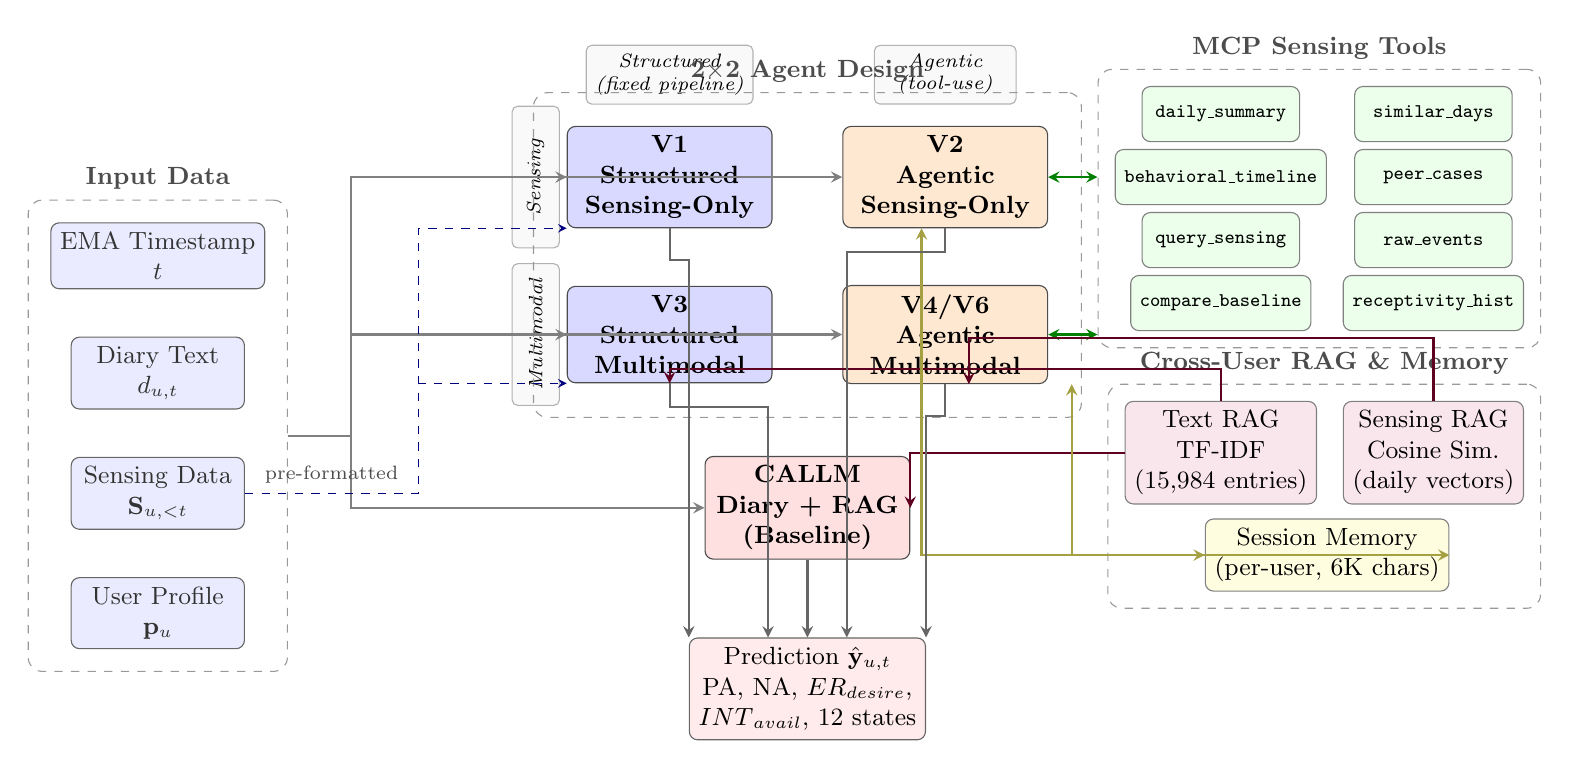
\begin{tikzpicture}[
    >=stealth,
    node distance=1.2cm and 1.8cm,
    % Style definitions
    databox/.style={rectangle, draw=black!60, fill=blue!8, rounded corners=3pt, minimum width=2.2cm, minimum height=0.8cm, font=\small, align=center, text=black!80},
    agentbox/.style={rectangle, draw=black!70, fill=orange!12, rounded corners=3pt, minimum width=2.6cm, minimum height=1cm, font=\small\bfseries, align=center},
    toolbox/.style={rectangle, draw=black!50, fill=green!8, rounded corners=3pt, minimum width=2cm, minimum height=0.7cm, font=\scriptsize, align=center},
    outputbox/.style={rectangle, draw=black!60, fill=red!8, rounded corners=3pt, minimum width=2.4cm, minimum height=0.8cm, font=\small, align=center},
    ragbox/.style={rectangle, draw=black!50, fill=purple!10, rounded corners=3pt, minimum width=2.2cm, minimum height=0.8cm, font=\small, align=center},
    membox/.style={rectangle, draw=black!50, fill=yellow!12, rounded corners=3pt, minimum width=2cm, minimum height=0.7cm, font=\small, align=center},
    groupbox/.style={rectangle, draw=black!40, dashed, rounded corners=5pt, inner sep=8pt},
    arrowlabel/.style={font=\scriptsize, text=black!70},
    dimbox/.style={rectangle, draw=black!30, fill=gray!5, rounded corners=2pt, minimum width=1.8cm, minimum height=0.6cm, font=\scriptsize\itshape, align=center},
]

% === LEFT: Input Data ===
\node[databox] (ema) at (0, 0) {EMA Timestamp\\$t$};
\node[databox, below=0.6cm of ema] (diary) {Diary Text\\$d_{u,t}$};
\node[databox, below=0.6cm of diary] (sensing) {Sensing Data\\$\mathbf{S}_{u,<t}$};
\node[databox, below=0.6cm of sensing] (profile) {User Profile\\$\mathbf{p}_u$};

% Group box around inputs
\node[groupbox, fit=(ema)(diary)(sensing)(profile), label={[font=\small\bfseries,text=black!70]above:Input Data}] (inputgroup) {};

% === CENTER: 2x2 Agent Design ===
% Structured column
\node[agentbox, fill=blue!15] (v1) at (6.5, 1) {V1\\Structured\\Sensing-Only};
\node[agentbox, fill=blue!15] (v3) at (6.5, -1) {V3\\Structured\\Multimodal};

% Agentic column
\node[agentbox, fill=orange!18] (v2) at (10, 1) {V2\\Agentic\\Sensing-Only};
\node[agentbox, fill=orange!18] (v4) at (10, -1) {V4/V6\\Agentic\\Multimodal};

% CALLM baseline
\node[agentbox, fill=red!12] (callm) at (8.25, -3.2) {CALLM\\Diary + RAG\\(Baseline)};

% Dimension labels
\node[dimbox] at (6.5, 2.3) {Structured\\(fixed pipeline)};
\node[dimbox] at (10, 2.3) {Agentic\\(tool-use)};
\node[dimbox, rotate=90, anchor=center] at (4.8, 1) {Sensing};
\node[dimbox, rotate=90, anchor=center] at (4.8, -1) {Multimodal};

% Group box around 2x2
\node[groupbox, fit=(v1)(v2)(v3)(v4), inner sep=12pt, label={[font=\small\bfseries,text=black!70]above:{2$\times$2 Agent Design}}] (designgroup) {};

% === BOTTOM-RIGHT: MCP Tools ===
\node[toolbox] (tool1) at (13.5, 1.8) {\texttt{daily\_summary}};
\node[toolbox] (tool2) at (13.5, 1.0) {\texttt{behavioral\_timeline}};
\node[toolbox] (tool3) at (13.5, 0.2) {\texttt{query\_sensing}};
\node[toolbox] (tool4) at (13.5, -0.6) {\texttt{compare\_baseline}};
\node[toolbox] (tool5) at (16.2, 1.8) {\texttt{similar\_days}};
\node[toolbox] (tool6) at (16.2, 1.0) {\texttt{peer\_cases}};
\node[toolbox] (tool7) at (16.2, 0.2) {\texttt{raw\_events}};
\node[toolbox] (tool8) at (16.2, -0.6) {\texttt{receptivity\_hist}};

\node[groupbox, fit=(tool1)(tool2)(tool3)(tool4)(tool5)(tool6)(tool7)(tool8), inner sep=6pt, label={[font=\small\bfseries,text=black!70]above:MCP Sensing Tools}] (toolgroup) {};

% === BOTTOM: RAG + Memory ===
\node[ragbox] (textrag) at (13.5, -2.5) {Text RAG\\TF-IDF\\(15,984 entries)};
\node[ragbox] (sensrag) at (16.2, -2.5) {Sensing RAG\\Cosine Sim.\\(daily vectors)};
\node[membox] (memory) at (14.85, -3.8) {Session Memory\\(per-user, 6K chars)};

\node[groupbox, fit=(textrag)(sensrag)(memory), inner sep=6pt, label={[font=\small\bfseries,text=black!70]above:Cross-User RAG \& Memory}] (raggroup) {};

% === RIGHT: Output ===
\node[outputbox] (output) at (8.25, -5.5) {Prediction $\hat{\mathbf{y}}_{u,t}$\\PA, NA, $\text{ER}_\text{desire}$,\\$\text{INT}_\text{avail}$, 12 states};

% === ARROWS ===
% Input to agents
\draw[->, thick, black!50] (inputgroup.east) -- ++(0.8,0) |- (v1.west);
\draw[->, thick, black!50] (inputgroup.east) -- ++(0.8,0) |- (v3.west);
\draw[->, thick, black!50] (inputgroup.east) -- ++(0.8,0) |- (v2.west);
\draw[->, thick, black!50] (inputgroup.east) -- ++(0.8,0) |- (v4.west);
\draw[->, thick, black!50] (inputgroup.east) -- ++(0.8,0) |- (callm.west);

% Agentic agents to tools (bidirectional)
\draw[<->, thick, green!50!black] (v2.east) -- (toolgroup.west |- v2);
\draw[<->, thick, green!50!black] (v4.east) -- (toolgroup.west |- v4);

% Structured agents get pre-formatted (one-way)
\draw[->, dashed, blue!50!black] (sensing.east) -- ++(2.2,0) node[arrowlabel, above, midway] {pre-formatted} |- (v1.south west);
\draw[->, dashed, blue!50!black] (sensing.east) -- ++(2.2,0) |- (v3.south west);

% RAG connections
\draw[->, thick, purple!50!black] (textrag.west) -| (callm.east);
\draw[->, thick, purple!50!black] (textrag.north) -- ++(0, 0.4) -| (v3.south);
\draw[->, thick, purple!50!black] (sensrag.north) -- ++(0, 0.8) -| ([xshift=3mm]v4.south);

% Memory connections
\draw[<->, thick, yellow!60!black] (memory.west) -| ([xshift=-3mm]v2.south);
\draw[<->, thick, yellow!60!black] (memory.east) -| ([xshift=3mm]v4.south east);

% Agents to output
\draw[->, thick, black!60] (v1.south) -- ++(0,-0.4) -| (output.north west);
\draw[->, thick, black!60] (v3.south) -- ++(0,-0.3) -| ([xshift=-5mm]output.north);
\draw[->, thick, black!60] (callm.south) -- (output.north);
\draw[->, thick, black!60] (v2.south) -- ++(0,-0.3) -| ([xshift=5mm]output.north);
\draw[->, thick, black!60] (v4.south) -- ++(0,-0.4) -| (output.north east);

\end{tikzpicture}
}
\caption{System architecture of the \sys{}. Input data (left) flows into a 2$\times$2 factorial design: \emph{structured} agents (V1, V3) receive pre-formatted sensing summaries in a single prompt, while \emph{agentic} agents (V2, V4/V6) autonomously query an MCP sensing server through tool-use. Cross-user RAG provides calibration anchors from 15,984 training entries. Agentic agents maintain per-user session memory across predictions. All variants produce the same structured prediction output.}
\label{fig:architecture}
\end{figure*}

\begin{figure*}[t]
\centering
\resizebox{\textwidth}{!}{%
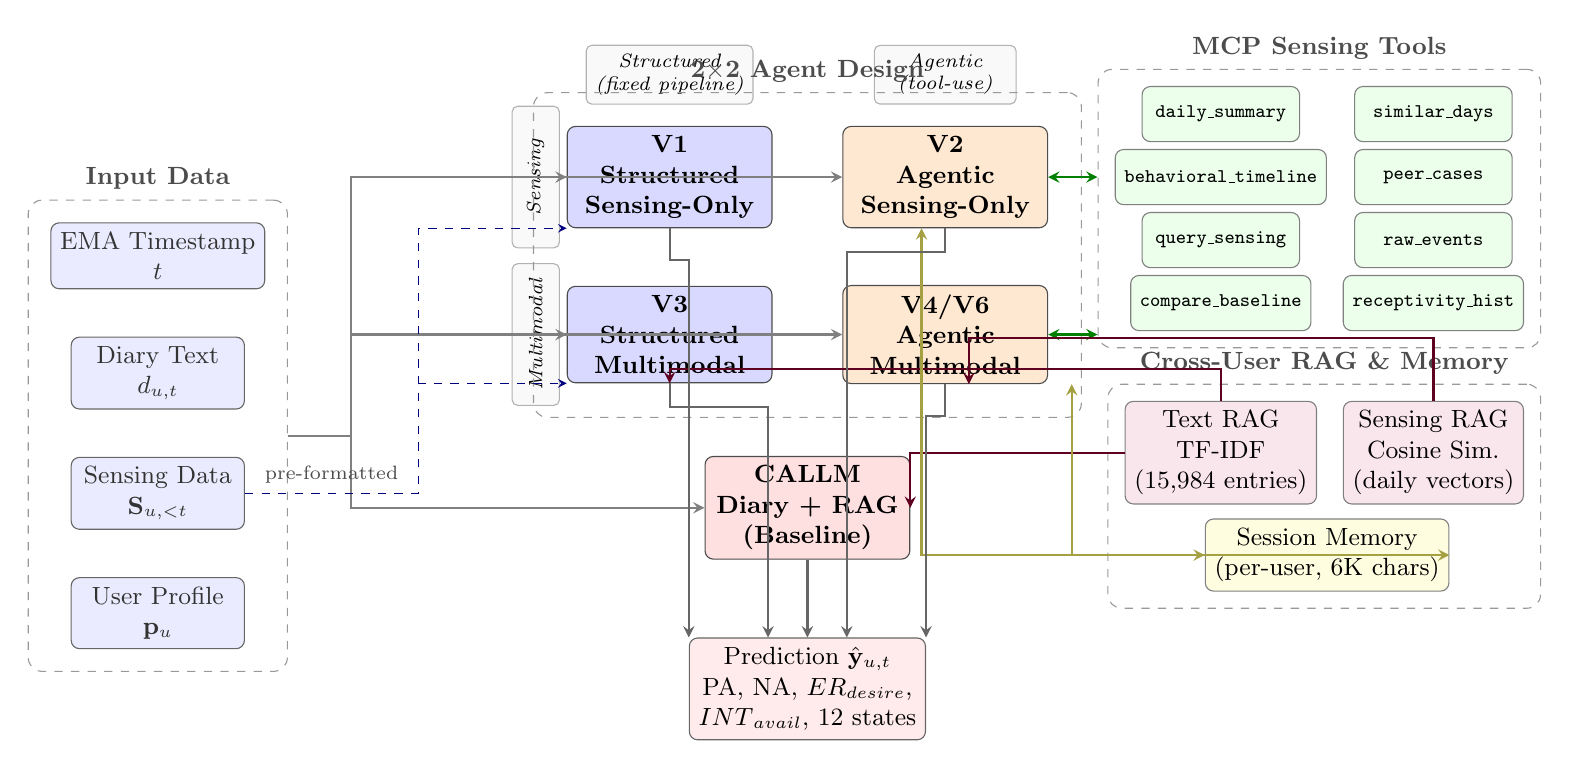
\begin{tikzpicture}[
    >=stealth,
    node distance=1.2cm and 1.8cm,
    % Style definitions
    databox/.style={rectangle, draw=black!60, fill=blue!8, rounded corners=3pt, minimum width=2.2cm, minimum height=0.8cm, font=\small, align=center, text=black!80},
    agentbox/.style={rectangle, draw=black!70, fill=orange!12, rounded corners=3pt, minimum width=2.6cm, minimum height=1cm, font=\small\bfseries, align=center},
    toolbox/.style={rectangle, draw=black!50, fill=green!8, rounded corners=3pt, minimum width=2cm, minimum height=0.7cm, font=\scriptsize, align=center},
    outputbox/.style={rectangle, draw=black!60, fill=red!8, rounded corners=3pt, minimum width=2.4cm, minimum height=0.8cm, font=\small, align=center},
    ragbox/.style={rectangle, draw=black!50, fill=purple!10, rounded corners=3pt, minimum width=2.2cm, minimum height=0.8cm, font=\small, align=center},
    membox/.style={rectangle, draw=black!50, fill=yellow!12, rounded corners=3pt, minimum width=2cm, minimum height=0.7cm, font=\small, align=center},
    groupbox/.style={rectangle, draw=black!40, dashed, rounded corners=5pt, inner sep=8pt},
    arrowlabel/.style={font=\scriptsize, text=black!70},
    dimbox/.style={rectangle, draw=black!30, fill=gray!5, rounded corners=2pt, minimum width=1.8cm, minimum height=0.6cm, font=\scriptsize\itshape, align=center},
]

% === LEFT: Input Data ===
\node[databox] (ema) at (0, 0) {EMA Timestamp\\$t$};
\node[databox, below=0.6cm of ema] (diary) {Diary Text\\$d_{u,t}$};
\node[databox, below=0.6cm of diary] (sensing) {Sensing Data\\$\mathbf{S}_{u,<t}$};
\node[databox, below=0.6cm of sensing] (profile) {User Profile\\$\mathbf{p}_u$};

% Group box around inputs
\node[groupbox, fit=(ema)(diary)(sensing)(profile), label={[font=\small\bfseries,text=black!70]above:Input Data}] (inputgroup) {};

% === CENTER: 2x2 Agent Design ===
% Structured column
\node[agentbox, fill=blue!15] (v1) at (6.5, 1) {V1\\Structured\\Sensing-Only};
\node[agentbox, fill=blue!15] (v3) at (6.5, -1) {V3\\Structured\\Multimodal};

% Agentic column
\node[agentbox, fill=orange!18] (v2) at (10, 1) {V2\\Agentic\\Sensing-Only};
\node[agentbox, fill=orange!18] (v4) at (10, -1) {V4/V6\\Agentic\\Multimodal};

% CALLM baseline
\node[agentbox, fill=red!12] (callm) at (8.25, -3.2) {CALLM\\Diary + RAG\\(Baseline)};

% Dimension labels
\node[dimbox] at (6.5, 2.3) {Structured\\(fixed pipeline)};
\node[dimbox] at (10, 2.3) {Agentic\\(tool-use)};
\node[dimbox, rotate=90, anchor=center] at (4.8, 1) {Sensing};
\node[dimbox, rotate=90, anchor=center] at (4.8, -1) {Multimodal};

% Group box around 2x2
\node[groupbox, fit=(v1)(v2)(v3)(v4), inner sep=12pt, label={[font=\small\bfseries,text=black!70]above:{2$\times$2 Agent Design}}] (designgroup) {};

% === BOTTOM-RIGHT: MCP Tools ===
\node[toolbox] (tool1) at (13.5, 1.8) {\texttt{daily\_summary}};
\node[toolbox] (tool2) at (13.5, 1.0) {\texttt{behavioral\_timeline}};
\node[toolbox] (tool3) at (13.5, 0.2) {\texttt{query\_sensing}};
\node[toolbox] (tool4) at (13.5, -0.6) {\texttt{compare\_baseline}};
\node[toolbox] (tool5) at (16.2, 1.8) {\texttt{similar\_days}};
\node[toolbox] (tool6) at (16.2, 1.0) {\texttt{peer\_cases}};
\node[toolbox] (tool7) at (16.2, 0.2) {\texttt{raw\_events}};
\node[toolbox] (tool8) at (16.2, -0.6) {\texttt{receptivity\_hist}};

\node[groupbox, fit=(tool1)(tool2)(tool3)(tool4)(tool5)(tool6)(tool7)(tool8), inner sep=6pt, label={[font=\small\bfseries,text=black!70]above:MCP Sensing Tools}] (toolgroup) {};

% === BOTTOM: RAG + Memory ===
\node[ragbox] (textrag) at (13.5, -2.5) {Text RAG\\TF-IDF\\(15,984 entries)};
\node[ragbox] (sensrag) at (16.2, -2.5) {Sensing RAG\\Cosine Sim.\\(daily vectors)};
\node[membox] (memory) at (14.85, -3.8) {Session Memory\\(per-user, 6K chars)};

\node[groupbox, fit=(textrag)(sensrag)(memory), inner sep=6pt, label={[font=\small\bfseries,text=black!70]above:Cross-User RAG \& Memory}] (raggroup) {};

% === RIGHT: Output ===
\node[outputbox] (output) at (8.25, -5.5) {Prediction $\hat{\mathbf{y}}_{u,t}$\\PA, NA, $\text{ER}_\text{desire}$,\\$\text{INT}_\text{avail}$, 12 states};

% === ARROWS ===
% Input to agents
\draw[->, thick, black!50] (inputgroup.east) -- ++(0.8,0) |- (v1.west);
\draw[->, thick, black!50] (inputgroup.east) -- ++(0.8,0) |- (v3.west);
\draw[->, thick, black!50] (inputgroup.east) -- ++(0.8,0) |- (v2.west);
\draw[->, thick, black!50] (inputgroup.east) -- ++(0.8,0) |- (v4.west);
\draw[->, thick, black!50] (inputgroup.east) -- ++(0.8,0) |- (callm.west);

% Agentic agents to tools (bidirectional)
\draw[<->, thick, green!50!black] (v2.east) -- (toolgroup.west |- v2);
\draw[<->, thick, green!50!black] (v4.east) -- (toolgroup.west |- v4);

% Structured agents get pre-formatted (one-way)
\draw[->, dashed, blue!50!black] (sensing.east) -- ++(2.2,0) node[arrowlabel, above, midway] {pre-formatted} |- (v1.south west);
\draw[->, dashed, blue!50!black] (sensing.east) -- ++(2.2,0) |- (v3.south west);

% RAG connections
\draw[->, thick, purple!50!black] (textrag.west) -| (callm.east);
\draw[->, thick, purple!50!black] (textrag.north) -- ++(0, 0.4) -| (v3.south);
\draw[->, thick, purple!50!black] (sensrag.north) -- ++(0, 0.8) -| ([xshift=3mm]v4.south);

% Memory connections
\draw[<->, thick, yellow!60!black] (memory.west) -| ([xshift=-3mm]v2.south);
\draw[<->, thick, yellow!60!black] (memory.east) -| ([xshift=3mm]v4.south east);

% Agents to output
\draw[->, thick, black!60] (v1.south) -- ++(0,-0.4) -| (output.north west);
\draw[->, thick, black!60] (v3.south) -- ++(0,-0.3) -| ([xshift=-5mm]output.north);
\draw[->, thick, black!60] (callm.south) -- (output.north);
\draw[->, thick, black!60] (v2.south) -- ++(0,-0.3) -| ([xshift=5mm]output.north);
\draw[->, thick, black!60] (v4.south) -- ++(0,-0.4) -| (output.north east);

\end{tikzpicture}
}
\caption{System architecture of the \sys{}. Input data (left) flows into a 2$\times$2 factorial design: \emph{structured} agents (V1, V3) receive pre-formatted sensing summaries in a single prompt, while \emph{agentic} agents (V2, V4/V6) autonomously query an MCP sensing server through tool-use. Cross-user RAG provides calibration anchors from 15,984 training entries. Agentic agents maintain per-user session memory across predictions. All variants produce the same structured prediction output.}
\label{fig:architecture}
\end{figure*}

\begin{figure*}[t]
\centering
\resizebox{\textwidth}{!}{%
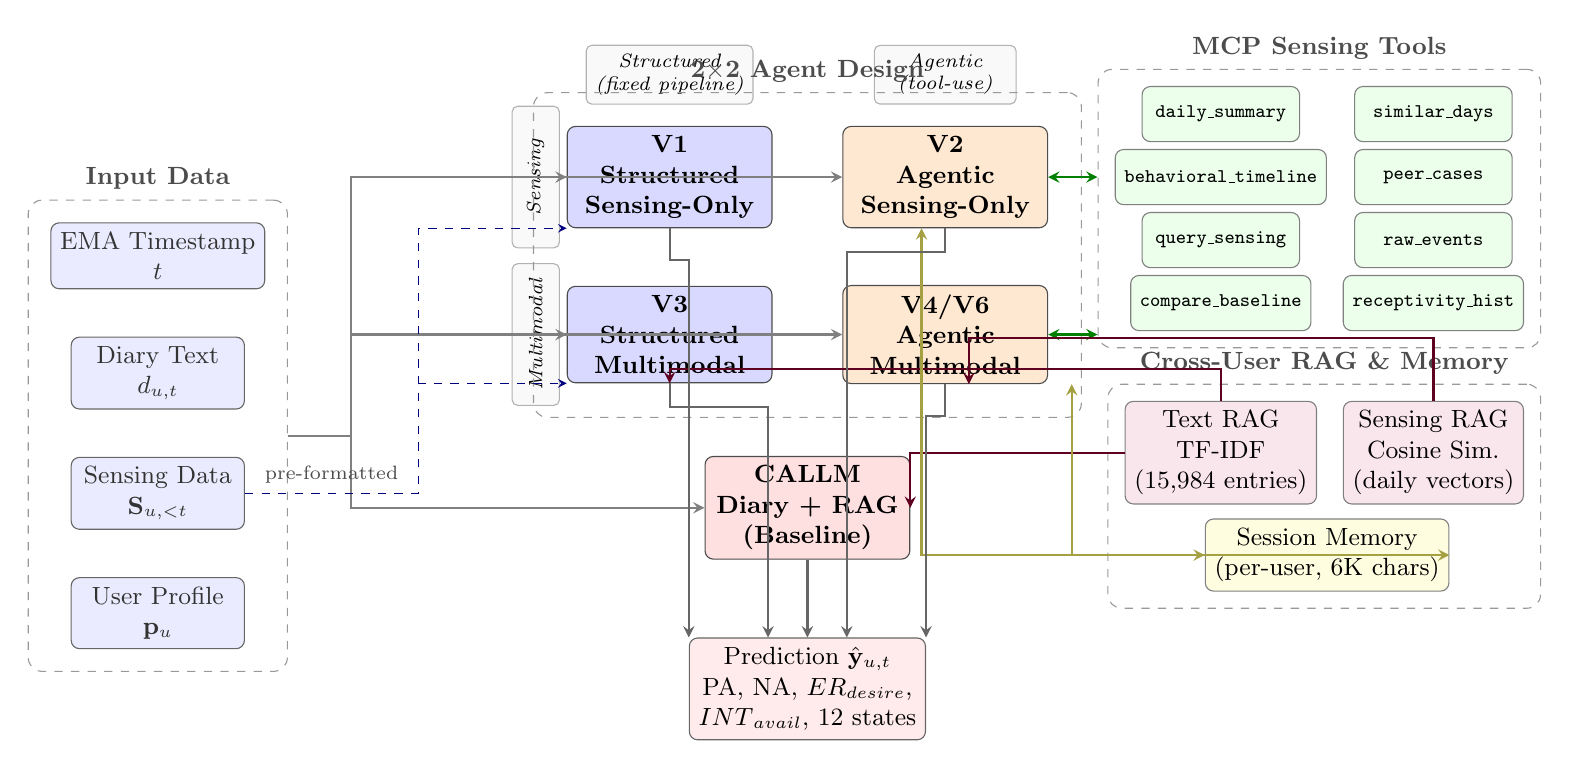
\begin{tikzpicture}[
    >=stealth,
    node distance=1.2cm and 1.8cm,
    % Style definitions
    databox/.style={rectangle, draw=black!60, fill=blue!8, rounded corners=3pt, minimum width=2.2cm, minimum height=0.8cm, font=\small, align=center, text=black!80},
    agentbox/.style={rectangle, draw=black!70, fill=orange!12, rounded corners=3pt, minimum width=2.6cm, minimum height=1cm, font=\small\bfseries, align=center},
    toolbox/.style={rectangle, draw=black!50, fill=green!8, rounded corners=3pt, minimum width=2cm, minimum height=0.7cm, font=\scriptsize, align=center},
    outputbox/.style={rectangle, draw=black!60, fill=red!8, rounded corners=3pt, minimum width=2.4cm, minimum height=0.8cm, font=\small, align=center},
    ragbox/.style={rectangle, draw=black!50, fill=purple!10, rounded corners=3pt, minimum width=2.2cm, minimum height=0.8cm, font=\small, align=center},
    membox/.style={rectangle, draw=black!50, fill=yellow!12, rounded corners=3pt, minimum width=2cm, minimum height=0.7cm, font=\small, align=center},
    groupbox/.style={rectangle, draw=black!40, dashed, rounded corners=5pt, inner sep=8pt},
    arrowlabel/.style={font=\scriptsize, text=black!70},
    dimbox/.style={rectangle, draw=black!30, fill=gray!5, rounded corners=2pt, minimum width=1.8cm, minimum height=0.6cm, font=\scriptsize\itshape, align=center},
]

% === LEFT: Input Data ===
\node[databox] (ema) at (0, 0) {EMA Timestamp\\$t$};
\node[databox, below=0.6cm of ema] (diary) {Diary Text\\$d_{u,t}$};
\node[databox, below=0.6cm of diary] (sensing) {Sensing Data\\$\mathbf{S}_{u,<t}$};
\node[databox, below=0.6cm of sensing] (profile) {User Profile\\$\mathbf{p}_u$};

% Group box around inputs
\node[groupbox, fit=(ema)(diary)(sensing)(profile), label={[font=\small\bfseries,text=black!70]above:Input Data}] (inputgroup) {};

% === CENTER: 2x2 Agent Design ===
% Structured column
\node[agentbox, fill=blue!15] (v1) at (6.5, 1) {V1\\Structured\\Sensing-Only};
\node[agentbox, fill=blue!15] (v3) at (6.5, -1) {V3\\Structured\\Multimodal};

% Agentic column
\node[agentbox, fill=orange!18] (v2) at (10, 1) {V2\\Agentic\\Sensing-Only};
\node[agentbox, fill=orange!18] (v4) at (10, -1) {V4/V6\\Agentic\\Multimodal};

% CALLM baseline
\node[agentbox, fill=red!12] (callm) at (8.25, -3.2) {CALLM\\Diary + RAG\\(Baseline)};

% Dimension labels
\node[dimbox] at (6.5, 2.3) {Structured\\(fixed pipeline)};
\node[dimbox] at (10, 2.3) {Agentic\\(tool-use)};
\node[dimbox, rotate=90, anchor=center] at (4.8, 1) {Sensing};
\node[dimbox, rotate=90, anchor=center] at (4.8, -1) {Multimodal};

% Group box around 2x2
\node[groupbox, fit=(v1)(v2)(v3)(v4), inner sep=12pt, label={[font=\small\bfseries,text=black!70]above:{2$\times$2 Agent Design}}] (designgroup) {};

% === BOTTOM-RIGHT: MCP Tools ===
\node[toolbox] (tool1) at (13.5, 1.8) {\texttt{daily\_summary}};
\node[toolbox] (tool2) at (13.5, 1.0) {\texttt{behavioral\_timeline}};
\node[toolbox] (tool3) at (13.5, 0.2) {\texttt{query\_sensing}};
\node[toolbox] (tool4) at (13.5, -0.6) {\texttt{compare\_baseline}};
\node[toolbox] (tool5) at (16.2, 1.8) {\texttt{similar\_days}};
\node[toolbox] (tool6) at (16.2, 1.0) {\texttt{peer\_cases}};
\node[toolbox] (tool7) at (16.2, 0.2) {\texttt{raw\_events}};
\node[toolbox] (tool8) at (16.2, -0.6) {\texttt{receptivity\_hist}};

\node[groupbox, fit=(tool1)(tool2)(tool3)(tool4)(tool5)(tool6)(tool7)(tool8), inner sep=6pt, label={[font=\small\bfseries,text=black!70]above:MCP Sensing Tools}] (toolgroup) {};

% === BOTTOM: RAG + Memory ===
\node[ragbox] (textrag) at (13.5, -2.5) {Text RAG\\TF-IDF\\(15,984 entries)};
\node[ragbox] (sensrag) at (16.2, -2.5) {Sensing RAG\\Cosine Sim.\\(daily vectors)};
\node[membox] (memory) at (14.85, -3.8) {Session Memory\\(per-user, 6K chars)};

\node[groupbox, fit=(textrag)(sensrag)(memory), inner sep=6pt, label={[font=\small\bfseries,text=black!70]above:Cross-User RAG \& Memory}] (raggroup) {};

% === RIGHT: Output ===
\node[outputbox] (output) at (8.25, -5.5) {Prediction $\hat{\mathbf{y}}_{u,t}$\\PA, NA, $\text{ER}_\text{desire}$,\\$\text{INT}_\text{avail}$, 12 states};

% === ARROWS ===
% Input to agents
\draw[->, thick, black!50] (inputgroup.east) -- ++(0.8,0) |- (v1.west);
\draw[->, thick, black!50] (inputgroup.east) -- ++(0.8,0) |- (v3.west);
\draw[->, thick, black!50] (inputgroup.east) -- ++(0.8,0) |- (v2.west);
\draw[->, thick, black!50] (inputgroup.east) -- ++(0.8,0) |- (v4.west);
\draw[->, thick, black!50] (inputgroup.east) -- ++(0.8,0) |- (callm.west);

% Agentic agents to tools (bidirectional)
\draw[<->, thick, green!50!black] (v2.east) -- (toolgroup.west |- v2);
\draw[<->, thick, green!50!black] (v4.east) -- (toolgroup.west |- v4);

% Structured agents get pre-formatted (one-way)
\draw[->, dashed, blue!50!black] (sensing.east) -- ++(2.2,0) node[arrowlabel, above, midway] {pre-formatted} |- (v1.south west);
\draw[->, dashed, blue!50!black] (sensing.east) -- ++(2.2,0) |- (v3.south west);

% RAG connections
\draw[->, thick, purple!50!black] (textrag.west) -| (callm.east);
\draw[->, thick, purple!50!black] (textrag.north) -- ++(0, 0.4) -| (v3.south);
\draw[->, thick, purple!50!black] (sensrag.north) -- ++(0, 0.8) -| ([xshift=3mm]v4.south);

% Memory connections
\draw[<->, thick, yellow!60!black] (memory.west) -| ([xshift=-3mm]v2.south);
\draw[<->, thick, yellow!60!black] (memory.east) -| ([xshift=3mm]v4.south east);

% Agents to output
\draw[->, thick, black!60] (v1.south) -- ++(0,-0.4) -| (output.north west);
\draw[->, thick, black!60] (v3.south) -- ++(0,-0.3) -| ([xshift=-5mm]output.north);
\draw[->, thick, black!60] (callm.south) -- (output.north);
\draw[->, thick, black!60] (v2.south) -- ++(0,-0.3) -| ([xshift=5mm]output.north);
\draw[->, thick, black!60] (v4.south) -- ++(0,-0.4) -| (output.north east);

\end{tikzpicture}
}
\caption{System architecture of the \sys{}. Input data (left) flows into a 2$\times$2 factorial design: \emph{structured} agents (V1, V3) receive pre-formatted sensing summaries in a single prompt, while \emph{agentic} agents (V2, V4/V6) autonomously query an MCP sensing server through tool-use. Cross-user RAG provides calibration anchors from 15,984 training entries. Agentic agents maintain per-user session memory across predictions. All variants produce the same structured prediction output.}
\label{fig:architecture}
\end{figure*}


\subsection{Problem Formulation}

Given a cancer survivor $u$ at EMA time $t$, we observe:
\begin{itemize}[nosep]
    \item \textbf{Sensing history} $\mathbf{S}_{u,<t}$: passive sensor data collected before time $t$ (motion, GPS, screen, keyboard, apps, light, music)
    \item \textbf{Diary text} $d_{u,t}$: optional free-text diary entry (present in $\sim$68\% of EMAs)
    \item \textbf{User profile} $\mathbf{p}_u$: trait questionnaire and demographic information
    \item \textbf{Memory} $\mathbf{m}_{u,<t}$: longitudinal context from prior predictions
\end{itemize}

\noindent The agent predicts a target vector $\hat{\mathbf{y}}_{u,t}$ comprising:
\begin{itemize}[nosep]
    \item \textbf{Continuous:} PANAS Positive Affect (0--30), PANAS Negative Affect (0--30), Emotion Regulation Desire (0--10)
    \item \textbf{Binary states:} Unusually elevated PA, NA, and 10 individual emotion states, plus \erdesire{} and \intavail{}
\end{itemize}

\noindent The binary ``state'' targets indicate whether each measure is at an \emph{unusual level for this individual} compared to their personal baseline---capturing personally meaningful deviations rather than absolute thresholds.

\subsection{2$\times$2 Factorial Design}

We systematically vary two design dimensions (Table~\ref{tab:design}):

\begin{table}[t]
\caption{The 2$\times$2 agent design space. Each cell represents a distinct agent architecture. CALLM serves as the diary-only baseline.}
\label{tab:design}
\small
\begin{tabular}{p{2cm}p{3.5cm}p{3.5cm}}
\toprule
& \textbf{Structured-Agentic} (fixed pipeline) & \textbf{Autonomously-Agentic} (autonomous tool-use) \\
\midrule
\textbf{Sensing-only} & Struct-Sense: Pre-formatted summary $\rightarrow$ 6-step reasoning & Auto-Sense/Auto-Sense+: MCP tools $\rightarrow$ autonomous investigation \\
\addlinespace
\textbf{Multimodal} (diary + sensing) & Struct-Multi: Diary + summary $\rightarrow$ 5-step reasoning & Auto-Multi/Auto-Multi+: Diary-first analysis $\rightarrow$ tool-based validation \\
\midrule
\multicolumn{3}{l}{\textbf{Baseline:} CALLM --- diary text + TF-IDF RAG, structured output~\cite{wang2026callm}} \\
\bottomrule
\end{tabular}
\end{table}

\paragraph{Dimension 1: Structured-Agentic vs.\ Autonomously-Agentic.}
\emph{Structured-agentic} agents (Struct-Sense, Struct-Multi) receive all relevant data as a pre-formatted text prompt and follow a fixed multi-step reasoning pipeline. This mirrors the dominant approach in prior work, where sensing features are pre-computed and presented to the model in a single context window.

\emph{Autonomously-agentic} agents (Auto-Sense, Auto-Multi, Auto-Multi+) receive the prediction task and a set of MCP tools (Section~\ref{sec:tools}), then autonomously decide which data to query, in what order, and how deeply to investigate. The agent reasons in a multi-turn loop---forming hypotheses, querying data, updating beliefs---before producing a final prediction. This mirrors how a behavioral data scientist might investigate a patient's daily patterns.

\paragraph{Dimension 2: Sensing-only vs.\ Multimodal.}
\emph{Sensing-only} agents (Struct-Sense, Auto-Sense) use exclusively passive sensor data---no diary text. This represents the fully proactive scenario where the system must predict emotional states without any active user input.

\emph{Multimodal} agents (Struct-Multi, Auto-Multi, Auto-Multi+) additionally receive the participant's diary entry, enabling cross-modal reasoning. The diary provides a ``ground truth'' emotional narrative that sensing tools can validate or contextualize.

\paragraph{Baseline: CALLM.}
The diary-only baseline~\cite{wang2026callm} uses the participant's diary text with TF-IDF retrieval-augmented generation to find similar cases from the training population. It represents the current state-of-the-art in LLM-based emotional state prediction for this population, but is fundamentally \emph{reactive}---it cannot operate when the diary is absent.

\subsection{Data: BUCS Cancer Survivorship Study}

We evaluate on data from the \emph{Behavioral Understanding for Cancer Survivors} (BUCS) study, a longitudinal investigation of 418 cancer survivors (297 iOS, 121 Android) over approximately 5 weeks. Participants completed EMAs three times daily (morning, afternoon, evening), yielding 15,984 total entries with the following:

\paragraph{EMA Targets.}
Each survey captures positive affect (PANAS-PA, sum of happy, cheerful, pleased, grateful; range 0--30), negative affect (PANAS-NA, sum of sad, afraid, miserable, worried, lonely; range 0--30), emotion regulation desire (0--10 scale), intervention availability (yes/no), and individual binary emotion states. Binary ``state'' labels are computed at the individual level: a participant's score is labeled as elevated if it exceeds their personal mean plus one standard deviation.

\paragraph{Diary Text.}
Approximately 68\% of EMA entries include a free-text \texttt{emotion\_driver} field describing the participant's current emotional experience. Entries range from brief (``fine'') to detailed narratives about health concerns, family events, or daily activities.

\paragraph{Passive Sensing (8 Modalities).}
Smartphones continuously collected data from 8 sensor streams, aggregated to hourly Parquet files:

\begin{enumerate}[nosep]
    \item \textbf{Motion/Accelerometer}: Stationary, walking, automotive, running durations; activity transitions
    \item \textbf{GPS/Mobility}: Travel distance and time, home time, max distance from home, location variance
    \item \textbf{Screen}: Unlock events, session counts, total and per-session durations
    \item \textbf{Keyboard}: Words typed, typing sessions, positive/negative sentiment ratios
    \item \textbf{App Usage} (Android only): Per-app foreground time, categorized (social, communication, entertainment)
    \item \textbf{Light} (Android only): Ambient light levels (lux)
    \item \textbf{Music}: Tracks played, listening duration, artists
    \item \textbf{Sleep}: Derived from accelerometer and Android sleep API
\end{enumerate}

\noindent Coverage varies by modality: motion and screen are available for nearly all participants, keyboard for 69\%, and app/light only for the 29\% on Android.

\paragraph{Data Splits.}
We use 5-fold across-subject cross-validation: all observations from a given participant appear in exactly one fold. The training set (80\% of participants) provides the population data for RAG and peer reference; the test set (20\%) provides evaluation data. LLM agents are evaluated on a subset of 50 test-set participants (${\sim}$3,900 EMA entries per condition) due to inference cost constraints.

\subsection{Structured-Agentic Architecture (Struct-Sense, Struct-Multi)}

Structured-agentic agents receive all data as a single pre-formatted prompt and follow a fixed reasoning pipeline in one LLM call.

\paragraph{Struct-Sense: Structured-Agentic Sensing-Only.}
The agent receives: (1) a natural-language summary of the day's sensing data (sleep, mobility, activity, screen, typing patterns), (2) the participant's trait profile and demographic information, (3) a longitudinal memory document tracking emotional patterns, and (4) peer reference cases---the 5 most similar behavioral profiles from the training population, retrieved via cosine similarity on daily sensing feature vectors, with their ground-truth EMA outcomes.

The agent follows a 6-step reasoning pipeline: (1) Sleep Analysis, (2) Mobility \& Activity, (3) Social Signals, (4) Pattern Integration, (5) Peer Comparison, (6) User Context $\rightarrow$ Final Prediction.

\paragraph{Struct-Multi: Structured-Agentic Multimodal.}
Extends Struct-Sense by adding the participant's diary text and multimodal RAG: the 10 most similar diary entries from the training set (via TF-IDF), enriched with each matched participant's sensing data and ground-truth outcomes. The agent follows a 5-step pipeline: (1) Diary Analysis, (2) Sensing Analysis, (3) Cross-Modal Consistency, (4) Similar Case Comparison, (5) Integrated Prediction.

\subsection{Autonomously-Agentic Architecture (Auto-Sense, Auto-Multi, Auto-Multi+)}
\label{sec:agentic}

Autonomously-agentic agents operate through a multi-turn tool-use loop. Each prediction spawns an LLM subprocess with access to an MCP server that exposes 8 sensing query tools backed by the participant's Parquet data store.

\paragraph{Auto-Sense: Autonomously-Agentic Sensing-Only.}
The agent receives a system prompt instructing it to investigate the participant's behavioral data like a ``behavioral data scientist detective,'' with a strategy: (1) reconstruct the day chronologically, (2) identify behavioral patterns, (3) detect anomalies via baseline comparison, (4) find analogous past days, (5) calibrate against peer cases, (6) synthesize into prediction. Critically, the agent \emph{decides which tools to call and in what order}---it may skip modalities it deems uninformative or drill deeply into anomalies.

\paragraph{Auto-Multi/Auto-Multi+: Autonomously-Agentic Multimodal.}
The agent additionally receives the diary entry and follows a \emph{diary-first} investigation strategy: (1) analyze diary text to extract emotional signals and form hypotheses, (2) use sensing tools to validate/calibrate those hypotheses, (3) check cross-modal consistency, (4) retrieve peer cases with similar diary content, (5) synthesize. The diary anchors the investigation, and sensing tools provide behavioral evidence for or against diary-derived hypotheses.

Auto-Multi+ additionally receives a pre-computed daily behavioral narrative---a filtered, structured summary of the day's sensing data with redundant and zero-information periods removed---reducing the raw data volume by 7.4$\times$ while preserving salient signals. We also evaluate Auto-Sense+, a sensing-only filtered variant (Auto-Sense + filtered narrative); Auto-Sense+ and Auto-Multi+ test whether data quality filtering improves prediction beyond the base autonomously-agentic approach.

% Agentic Investigation Flow Figure
% Shows the multi-turn reasoning loop for V4/V6
\begin{figure}[t]
\centering
\resizebox{\columnwidth}{!}{%
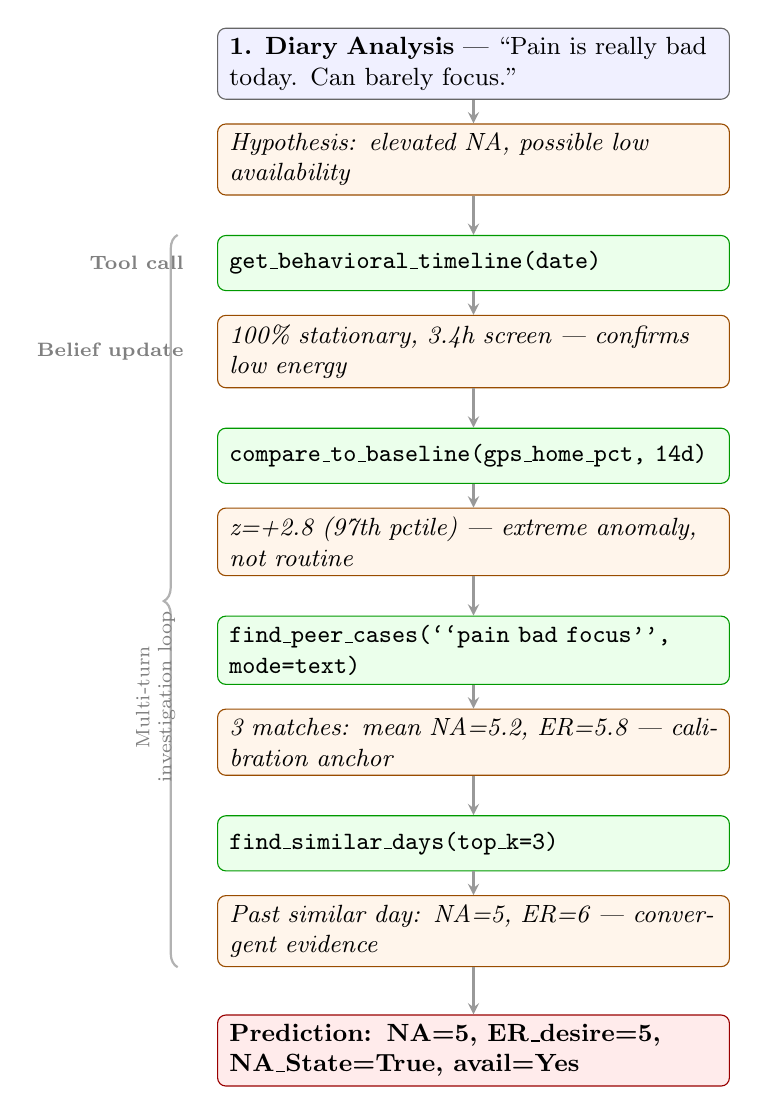
\begin{tikzpicture}[
    >=stealth,
    node distance=0.8cm,
    stepbox/.style={rectangle, draw=black!60, fill=blue!6, rounded corners=3pt, minimum width=6.5cm, minimum height=0.7cm, font=\small, align=left, text width=6.2cm},
    toolcall/.style={rectangle, draw=green!60!black, fill=green!8, rounded corners=3pt, minimum width=6.5cm, minimum height=0.7cm, font=\small\ttfamily, align=left, text width=6.2cm},
    belief/.style={rectangle, draw=orange!60!black, fill=orange!8, rounded corners=3pt, minimum width=6.5cm, minimum height=0.6cm, font=\small\itshape, align=left, text width=6.2cm},
    resultbox/.style={rectangle, draw=red!60!black, fill=red!8, rounded corners=3pt, minimum width=6.5cm, minimum height=0.7cm, font=\small\bfseries, align=left, text width=6.2cm},
    looplabel/.style={font=\scriptsize\bfseries, text=black!50},
]

% Step 1: Diary analysis
\node[stepbox] (s1) at (0, 0) {\textbf{1. Diary Analysis} --- ``Pain is really bad today. Can barely focus.''};
\node[belief, below=0.3cm of s1] (b1) {Hypothesis: elevated NA, possible low availability};

% Step 2: Timeline
\node[toolcall, below=0.5cm of b1] (t2) {get\_behavioral\_timeline(date)};
\node[belief, below=0.3cm of t2] (b2) {100\% stationary, 3.4h screen --- confirms low energy};

% Step 3: Baseline comparison
\node[toolcall, below=0.5cm of b2] (t3) {compare\_to\_baseline(gps\_home\_pct, 14d)};
\node[belief, below=0.3cm of t3] (b3) {z=+2.8 (97th pctile) --- extreme anomaly, not routine};

% Step 4: Peer cases
\node[toolcall, below=0.5cm of b3] (t4) {find\_peer\_cases(``pain bad focus'', mode=text)};
\node[belief, below=0.3cm of t4] (b4) {3 matches: mean NA=5.2, ER=5.8 --- calibration anchor};

% Step 5: Similar days
\node[toolcall, below=0.5cm of b4] (t5) {find\_similar\_days(top\_k=3)};
\node[belief, below=0.3cm of t5] (b5) {Past similar day: NA=5, ER=6 --- convergent evidence};

% Final prediction
\node[resultbox, below=0.6cm of b5] (pred) {Prediction: NA=5, ER\_desire=5, NA\_State=True, avail=Yes};

% Arrows
\foreach \a/\b in {s1/b1, b1/t2, t2/b2, b2/t3, t3/b3, b3/t4, t4/b4, b4/t5, t5/b5, b5/pred} {
    \draw[->, thick, black!40] (\a.south) -- (\b.north);
}

% Loop annotations
\node[looplabel, left=0.3cm of t2] {Tool call};
\node[looplabel, left=0.3cm of b2] {Belief update};

% Brace for multi-turn loop
\draw[decorate, decoration={brace, amplitude=5pt, mirror}, thick, black!30]
    ([xshift=-0.5cm]t2.north west) -- ([xshift=-0.5cm]b5.south west)
    node[midway, left=8pt, font=\scriptsize, text=black!50, align=center, rotate=90] {Multi-turn\\investigation loop};

\end{tikzpicture}
}
\caption{Example agentic investigation trace (V4, Participant 071). The agent analyzes the diary entry, forms a hypothesis, then autonomously queries sensing tools to validate and calibrate. Each tool call updates the agent's belief state. The investigation converges after 5 tool calls with cross-validated evidence from behavioral data, peer cases, and historical patterns.}
\label{fig:agentic_flow}
\end{figure}


\paragraph{Session Memory.}
Agentic agents maintain per-user longitudinal memory across predictions. After each prediction, the agent generates a 1--2 sentence ``reflection'' capturing calibration lessons (e.g., ``this user's self-reported negative affect is typically lower than behavioral signals suggest''). Reflections accumulate into a session memory document, capped at 6,000 characters. To prevent ground-truth leakage, reflections reference only receptivity signals (diary themes, \erdesire{}, \intavail{})---never PANAS scores.

\subsection{Sensing Query Tools (MCP Server)}
\label{sec:tools}

Our tool design is grounded in two principles from behavioral science and mobile sensing. First, clinical reasoning in psychological assessment follows a hypothesis-driven process: clinicians begin with an overview, form hypotheses, then seek confirming and disconfirming evidence through targeted investigation~\cite{wilcox2023clinical_reasoning}. Our tools mirror this workflow, progressing from broad summaries (\texttt{get\_daily\_summary}) to targeted queries (\texttt{query\_sensing}, \texttt{query\_raw\_events}). Second, idiographic (person-specific) analysis consistently outperforms nomothetic (population-level) models for affect prediction from behavioral data~\cite{beltz2016idiographic, balliu2024personalized_mood}---Balliu et al.\ showed that personalized smartphone-based mood models achieve $R^2 \geq 0.80$ compared to $< 0.05$ for population models. We therefore provide tools for personalized baseline comparison (\texttt{compare\_to\_baseline}), within-person analogical retrieval (\texttt{find\_similar\_days}), and cross-user calibration (\texttt{find\_peer\_cases}). This design also follows the multi-step health data investigation paradigm validated by PHIA~\cite{merrill2025phia}, which demonstrated that agentic multi-step reasoning over wearable data substantially outperforms single-pass analysis.

The MCP server exposes 8 tools, each querying the participant's hourly Parquet data store. The agent calls these tools autonomously during its investigation:

\begin{enumerate}[nosep]
    \item \texttt{get\_daily\_summary}: Full-day behavioral overview across all modalities
    \item \texttt{get\_behavioral\_timeline}: Chronological day reconstruction with 3--6 hour segments and behavioral-state labels with cautious affective cues
    \item \texttt{query\_sensing}: Targeted hourly query by modality, time window, and duration
    \item \texttt{query\_raw\_events}: Raw event streams (exact lock/unlock times, app sessions, motion transitions, typed text, songs played)
    \item \texttt{compare\_to\_baseline}: Z-score comparison against this user's 14-day historical mean/SD; flags behavioral anomalies
    \item \texttt{get\_receptivity\_history}: Past 14 days of intervention accept/reject patterns plus aggregate mood trends
    \item \texttt{find\_similar\_days}: Cosine similarity on daily sensing vectors; returns 5 most behaviorally similar past days with ground-truth outcomes
    \item \texttt{find\_peer\_cases}: Cross-user search over training population. Text mode: TF-IDF on diary text. Sensing mode: cosine similarity on daily behavioral fingerprints. Returns peer cases with ground-truth outcomes as calibration anchors.
\end{enumerate}

\noindent Agents are limited to 16 tool calls per prediction (timeout: 600 seconds). In practice, agents typically use 4--8 calls, demonstrating selective investigation.

\subsection{Cross-User Retrieval-Augmented Generation}

A key challenge in affect prediction is calibration: how does the agent know what absolute PANAS values correspond to the behavioral patterns it observes? We address this through \emph{cross-user RAG}, which retrieves similar cases from a peer database of 15,984 training-set EMA entries (96\% with associated sensing data). The retrieved cases provide ground-truth outcomes that serve as calibration anchors.

Three retrieval modes serve different agent configurations:
\begin{itemize}[nosep]
    \item \textbf{Text retrieval} (CALLM, Struct-Multi, Auto-Multi/Auto-Multi+): TF-IDF similarity over diary text (5,000 features, bigrams, min document frequency 2). Returns 10--20 most similar diary entries with outcomes.
    \item \textbf{Sensing retrieval} (Struct-Sense, Auto-Sense): Cosine similarity on z-score normalized daily sensing feature vectors. Returns 5 most behaviorally similar peer days with outcomes.
    \item \textbf{Tool-based retrieval} (Auto-Sense, Auto-Multi/Auto-Multi+): The \texttt{find\_peer\_cases} MCP tool exposes both modes to autonomously-agentic agents, letting them choose retrieval strategy.
\end{itemize}

\noindent Current-participant entries are excluded from retrieval to prevent data leakage.


%% ================================================================
%%  4. EVALUATION METHODOLOGY
%% ================================================================
\section{Evaluation Methodology}

\subsection{Evaluation Setup}

We evaluate all agent variants on 50 cancer survivors drawn from the BUCS test sets. These participants span all 5 cross-validation folds, yielding approximately 3,900 EMA entries per agent variant (3,851--3,955 depending on version-specific parsing). Each participant contributes 70--96 chronologically ordered EMA entries, evaluated sequentially to simulate real-time deployment. The 50 participants were randomly sampled from the test folds and do not differ significantly from the full 418-participant cohort on the key prediction targets (PA\_State, \erdesire{}, \intavail{} base rates, mean positive affect; Mann-Whitney $p > 0.05$), though the subset shows slightly lower negative affect prevalence ($p = 0.028$, $r = 0.19$) and a higher proportion of Android users (42\% vs.\ 25\%), both with small effect sizes.

\subsection{Baselines}

\paragraph{Traditional ML.}
Random Forest (RF) and XGBoost classifiers/regressors trained on 20 daily aggregate sensing features via 5-fold across-subject CV on the full dataset (15,984 entries), with held-out predictions filtered to the same 50 evaluation participants for fair comparison. Additional variants include logistic regression and MLP.

\paragraph{Text Baselines.}
TF-IDF + SVM, Bag-of-Words + SVM, and MiniLM sentence transformer embeddings + SVM, all trained on diary text via 5-fold CV.

\paragraph{Combined Baselines.}
RF and logistic regression trained on concatenated sensing features and diary text embeddings.

\subsection{Metrics}

We report two classes of metrics aligned with our prediction targets:

\paragraph{Binary State Targets.}
\emph{Balanced Accuracy} (BA = (TPR + TNR) / 2) handles the class imbalance inherent in ``unusual state'' detection (most entries are not elevated). \emph{Macro F1} provides a complementary measure. We report per-target and mean values across all binary targets. We focus exclusively on binary classification metrics, as the clinically actionable question is whether a state is \emph{elevated or not}, rather than the exact numeric value.

\paragraph{Focus Targets.}
Per the study's emphasis on intervention opportunity and affect, we highlight: \erdesire{} (continuous and binary), \intavail{} (binary), PA\_State, and NA\_State. Remaining targets (individual emotions, pain, forecasting, interactions quality) are reported in the appendix.

\paragraph{Class Balance.}
The binary state targets exhibit varying base rates across the 50 participants: PA\_State is nearly balanced (54.7\% elevated), while NA\_State (31.2\%), \erdesire{} State (34.4\%), and individual negative emotions (28--33\%) are moderately imbalanced. \intavail{} is 66.2\% positive overall but varies dramatically across individuals, reflecting genuine heterogeneity in availability patterns. These base rates motivate our use of balanced accuracy, which accounts for class imbalance.

\subsection{Implementation}

All LLM agents use Claude Sonnet (claude-sonnet-4-6) via the Claude Max subscription, with no API cost. Structured-agentic agents (Struct-Sense, Struct-Multi, CALLM) use \texttt{claude -p} (single-call mode); autonomously-agentic agents (Auto-Sense, Auto-Multi, Auto-Multi+) use \texttt{claude --print} with an MCP server subprocess. Concurrent processes are limited to 5 to respect subscription rate limits. Each autonomously-agentic prediction typically takes 30--90 seconds and uses 4--8 tool calls. Full system prompts and MCP tool definitions will be released upon publication to support reproducibility.


%% ================================================================
%%  5. RESULTS
%% ================================================================
\section{Results}

\subsection{Overview: Aggregate Performance}

Table~\ref{tab:main_results} and Figure~\ref{fig:ba_comparison} present aggregate results across all prediction targets. The autonomously-agentic multimodal variants (Auto-Multi, Auto-Multi+) achieve the highest overall balanced accuracy and F1.

\begin{table}[t]
\caption{Aggregate performance across all prediction targets (50 users, ${\sim}$3,900 entries per variant). Best in each column is \textbf{bold}. $\dagger$ML baselines trained via 5-fold CV on the full dataset; predictions filtered to the same 50 evaluation users.}
\label{tab:main_results}
\small
\begin{tabular}{llcc}
\toprule
\textbf{System} & \textbf{Input} & \textbf{Mean BA}$\uparrow$ & \textbf{Mean F1}$\uparrow$ \\
\midrule
\multicolumn{4}{l}{\emph{LLM Agent Systems}} \\
CALLM & Diary + RAG & 0.611 & 0.594 \\
Struct-Sense & Sensing & 0.516 & 0.428 \\
Auto-Sense & Sensing & 0.589 & 0.583 \\
Auto-Sense+ & Sensing (filtered) & 0.591 & 0.584 \\
Struct-Multi & Multimodal & 0.603 & 0.584 \\
Auto-Multi & Multimodal & 0.660 & \textbf{0.657} \\
Auto-Multi+ & Multimodal (filtered) & \textbf{0.661} & 0.656 \\
\addlinespace
\multicolumn{4}{l}{\emph{Baselines}$^\dagger$} \\
MiniLM & Diary embed. & 0.629 & 0.588 \\
TF-IDF + SVM & Diary text & 0.613 & 0.570 \\
Combined RF & Sensing + diary & 0.620 & 0.568 \\
RF & Sensing & 0.501 & 0.365 \\
XGBoost & Sensing & 0.502 & 0.391 \\
\bottomrule
\end{tabular}
\end{table}

\input{figures/results_ba_comparison}

The overall ranking is: autonomously-agentic multimodal (Auto-Multi+/Auto-Multi) $>$ structured-agentic multimodal (Struct-Multi) $>$ CALLM $>$ autonomously-agentic sensing (Auto-Sense+/Auto-Sense) $>$ text baselines $>$ structured-agentic sensing (Struct-Sense) $>$ ML sensing baselines. The autonomously-agentic multimodal agents (Auto-Multi+: BA=0.661, Auto-Multi: BA=0.660) outperform the best traditional baseline (MiniLM BA=0.629), though this comparison is confounded by the richer data access available to LLM agents (Section~\ref{sec:tools}). The more controlled comparison---agentic vs.\ structured within the same LLM and data access framework---shows consistent and statistically significant improvements (Section~\ref{sec:results_agentic}).

\subsection{Intervention Opportunity: Desire and Availability}
\label{sec:results_intervention}

Table~\ref{tab:intervention} and Figure~\ref{fig:intervention_bars} present results for the two components of intervention opportunity.

\begin{table}[t]
\caption{Intervention opportunity prediction (50 users). \erdesire{}: emotion regulation desire; \intavail{}: intervention availability. Best per metric is \textbf{bold}.}
\label{tab:intervention}
\small
\begin{tabular}{l cc cc}
\toprule
& \multicolumn{2}{c}{\erdesire{} State (Binary)} & \multicolumn{2}{c}{\intavail{} (Binary)} \\
\textbf{System} & BA & F1 & BA & F1 \\
\midrule
CALLM & 0.632 & 0.635 & 0.542 & 0.532 \\
Struct-Sense & 0.508 & 0.444 & 0.533 & 0.490 \\
Auto-Sense & 0.652 & 0.656 & 0.706 & 0.713 \\
Auto-Sense+ & 0.653 & 0.658 & 0.685 & 0.693 \\
Struct-Multi & 0.664 & 0.674 & 0.551 & 0.546 \\
Auto-Multi & 0.745 & 0.752 & \textbf{0.716} & \textbf{0.717} \\
Auto-Multi+ & \textbf{0.751} & \textbf{0.758} & 0.707 & 0.710 \\
\midrule
MiniLM$^\dagger$ & 0.629 & 0.588 & 0.573 & 0.624 \\
RF$^\dagger$ & 0.501 & 0.365 & --- & --- \\
\bottomrule
\end{tabular}
\end{table}

\input{figures/results_intervention}

\paragraph{Emotion Regulation Desire.}
Detecting when a cancer survivor \emph{wants} emotional support is the most direct signal for intervention timing. The autonomously-agentic multimodal agents achieve strong performance: Auto-Multi+ attains BA = 0.751 and Auto-Multi BA = 0.745, outperforming both the structured-agentic multimodal agent (Struct-Multi: BA = 0.664) and CALLM (BA = 0.632). The autonomously-agentic sensing-only agent (Auto-Sense: BA = 0.652) also outperforms Struct-Sense (BA = 0.508), demonstrating the value of autonomous investigation even without diary text.

\paragraph{Intervention Availability.}
Predicting whether a survivor is \emph{available} to engage with an intervention shows a striking pattern: autonomously-agentic agents significantly outperform structured-agentic ones. Auto-Multi (BA = 0.716) and Auto-Multi+ (BA = 0.707) exceed Struct-Multi (BA = 0.551) and CALLM (BA = 0.542). Even the sensing-only agent Auto-Sense (BA = 0.706) outperforms all structured variants. Interestingly, the filtered variants slightly regress on availability (Auto-Sense+: 0.685 vs.\ Auto-Sense: 0.706; Auto-Multi+: 0.707 vs.\ Auto-Multi: 0.716), suggesting that the behavioral narrative filtering may remove signals relevant to availability detection (e.g., raw screen unlock patterns or motion transitions). This finding indicates that \emph{behavioral signals}---detectable through autonomous sensing investigation---are more informative for availability prediction than diary text alone.

\paragraph{Intervention Opportunity (Joint Prediction).}
For a JITAI to act, both desire and availability must be predicted correctly. We evaluate the joint prediction where both \erdesire{} State = True \emph{and} \intavail{} = yes. The autonomously-agentic multimodal agents achieve the best joint detection, substantially outperforming CALLM and structured variants. This confirms that agentic multimodal agents excel not just on individual constructs but on the clinically actionable conjunction. In contrast, CALLM performs well on desire (0.632) but poorly on availability (0.542), causing it to miss the joint opportunity.

\subsection{Positive and Negative Affect}
\label{sec:results_affect}

Table~\ref{tab:affect} presents results for affect state detection and continuous prediction.

\begin{table}[t]
\caption{Affect state detection (50 users). PA/NA State: binary (elevated vs.\ typical). Best per metric is \textbf{bold}.}
\label{tab:affect}
\small
\begin{tabular}{l cc cc}
\toprule
& \multicolumn{2}{c}{PA State} & \multicolumn{2}{c}{NA State} \\
\textbf{System} & BA & F1 & BA & F1 \\
\midrule
CALLM & 0.534 & 0.466 & 0.641 & 0.652 \\
Struct-Sense & 0.505 & 0.330 & 0.510 & 0.460 \\
Auto-Sense & 0.598 & 0.597 & 0.592 & 0.586 \\
Auto-Sense+ & 0.595 & 0.594 & 0.601 & 0.593 \\
Struct-Multi & 0.533 & 0.466 & 0.674 & 0.688 \\
Auto-Multi & 0.724 & 0.725 & 0.716 & 0.712 \\
Auto-Multi+ & \textbf{0.733} & \textbf{0.734} & \textbf{0.722} & \textbf{0.715} \\
\midrule
MiniLM$^\dagger$ & 0.689 & 0.709 & 0.680 & 0.580 \\
\bottomrule
\end{tabular}
\end{table}

\paragraph{Negative Affect State Detection.}
Detecting elevated negative affect---the strongest clinical signal for intervention need---is where agentic multimodal agents shine. Auto-Multi+ achieves BA = 0.722, above Struct-Multi (0.674) and CALLM (0.641). This represents a meaningful improvement: at 72\% balanced accuracy, the system correctly identifies nearly 3 out of 4 instances of elevated negative affect, while maintaining a low false positive rate.

\paragraph{Positive Affect State Detection.}
Detecting unusual positive affect states follows the same pattern. Auto-Multi+ (BA = 0.733) substantially outperforms Struct-Multi (0.533) and CALLM (0.534). Positive affect tracking is valuable for identifying moments of resilience and wellbeing that can be reinforced through positive psychology interventions.


\subsection{Structured vs.\ Agentic: The Value of Autonomous Investigation}
\label{sec:results_agentic}

Table~\ref{tab:agentic_vs_structured} isolates the effect of agentic reasoning by comparing matched pairs within each data condition.

\begin{table}[t]
\caption{Effect of agentic reasoning (50 users). $\Delta$ = agentic $-$ structured (positive = agentic better). Results on focus targets.}
\label{tab:agentic_vs_structured}
\small
\begin{tabular}{l cc cc}
\toprule
& \multicolumn{2}{c}{Sensing-Only} & \multicolumn{2}{c}{Multimodal} \\
\textbf{Target (BA)} & Struct-Sense & Auto-Sense & Struct-Multi & Auto-Multi \\
\midrule
\erdesire{} State & 0.508 & \textbf{0.652} {\scriptsize (+.144)} & 0.664 & \textbf{0.745} {\scriptsize (+.081)} \\
\intavail{} & 0.533 & \textbf{0.706} {\scriptsize (+.173)} & 0.551 & \textbf{0.716} {\scriptsize (+.165)} \\
PA State & 0.505 & \textbf{0.598} {\scriptsize (+.093)} & 0.533 & \textbf{0.724} {\scriptsize (+.191)} \\
NA State & 0.510 & \textbf{0.592} {\scriptsize (+.082)} & 0.674 & \textbf{0.716} {\scriptsize (+.042)} \\
\addlinespace
Mean BA (all) & 0.516 & \textbf{0.589} {\scriptsize (+.073)} & 0.603 & \textbf{0.660} {\scriptsize (+.057)} \\
\bottomrule
\end{tabular}
\end{table}

The agentic approach consistently and substantially outperforms the structured approach across all targets and both data conditions. The improvement is especially dramatic for:

\begin{itemize}[nosep]
    \item \textbf{Intervention availability} (+0.173 BA in sensing-only, +0.165 in multimodal): Availability depends on contextual behavioral signals (current activity, time patterns) that benefit from selective investigation. Structured agents receive all features equally weighted, while agentic agents can focus on the specific signals (screen activity, motion state, time of day) most relevant to availability.

    \item \textbf{Positive affect in multimodal} (+0.191 BA): The largest single improvement, suggesting that agentic investigation is particularly valuable for detecting positive emotional states when diary text provides initial hypotheses that sensing data can validate.

    \item \textbf{Sensing-only condition} (+0.073 overall BA): When no diary text is available, the agentic approach's ability to selectively investigate sensor streams becomes more valuable. The structured agent receives a flat feature summary that treats all modalities equally; the agentic agent can recognize, for example, that a day of unusually low mobility warrants deeper GPS investigation while ignoring unexceptional screen patterns.
\end{itemize}

The improvement is smaller (but still consistent) in the multimodal condition, where the diary text already provides a strong signal that reduces the marginal value of autonomous sensing investigation.

\paragraph{Per-User Consistency and Statistical Significance.}
The agentic advantage is not driven by outlier participants. We compute per-user mean BA across all binary targets for each of the 50 participants and compare agent variants using paired Wilcoxon signed-rank tests. Auto-Multi significantly outperforms Struct-Multi on mean BA ($p < 10^{-11}$, $r = 0.95$) and CALLM ($p < 10^{-11}$, $r = 0.93$); Auto-Sense significantly outperforms Struct-Sense ($p < 10^{-10}$, $r = 0.91$). All four focus targets show significant improvements for Auto-Multi over Struct-Multi: PA~State ($p < 10^{-9}$), NA~State ($p < 10^{-5}$), \erdesire{}~State ($p = 0.014$), and \intavail{} ($p = 0.046$). Bootstrap 95\% confidence intervals for per-user mean BA confirm non-overlapping intervals: Auto-Multi $[0.634, 0.658]$, Auto-Multi+ $[0.631, 0.657]$, vs.\ Struct-Multi $[0.592, 0.616]$ and CALLM $[0.601, 0.621]$.

\subsection{Sensing-Only vs.\ Multimodal}
\label{sec:results_modality}

\begin{table}[t]
\caption{Effect of data modality (50 users). $\Delta$ = multimodal $-$ sensing-only (positive = multimodal better).}
\label{tab:modality}
\small
\begin{tabular}{l cc cc}
\toprule
& \multicolumn{2}{c}{Structured} & \multicolumn{2}{c}{Agentic} \\
\textbf{Target (BA)} & Struct-Sense & Struct-Multi & Auto-Sense & Auto-Multi \\
\midrule
\erdesire{} State & 0.508 & \textbf{0.664} {\scriptsize (+.156)} & 0.652 & \textbf{0.745} {\scriptsize (+.093)} \\
\intavail{} & 0.533 & 0.551 {\scriptsize (+.018)} & \textbf{0.706} & \textbf{0.716} {\scriptsize (+.010)} \\
PA State & 0.505 & 0.533 {\scriptsize (+.028)} & 0.598 & \textbf{0.724} {\scriptsize (+.126)} \\
NA State & 0.510 & \textbf{0.674} {\scriptsize (+.164)} & 0.592 & \textbf{0.716} {\scriptsize (+.124)} \\
\addlinespace
Mean BA (all) & 0.516 & 0.603 {\scriptsize (+.087)} & 0.589 & \textbf{0.660} {\scriptsize (+.071)} \\
\bottomrule
\end{tabular}
\end{table}

Adding diary text to sensing data consistently improves performance, with particularly large gains for affect-related targets (NA State: +0.164 in structured, +0.124 in agentic). Diary text provides direct emotional content that is difficult to infer from behavioral signals alone. However, the improvement for \intavail{} is minimal in both conditions (+0.018 structured, +0.010 agentic), confirming that availability is primarily a behavioral construct well-captured by sensing data.

\subsection{Calibration Analysis}

\begin{table}[t]
\caption{Prediction calibration for continuous targets (50 users). We report predicted vs.\ ground truth distribution statistics. Well-calibrated systems have similar mean and standard deviation.}
\label{tab:calibration}
\small
\begin{tabular}{l cccc}
\toprule
\textbf{System} & \textbf{PA pred $\mu$/$\sigma$} & \textbf{PA GT $\mu$/$\sigma$} & \textbf{NA pred $\mu$/$\sigma$} & \textbf{NA GT $\mu$/$\sigma$} \\
\midrule
Auto-Multi+ & 16.0 / 4.9 & 18.1 / 8.2 & 9.1 / 4.9 & 3.1 / 4.9 \\
Auto-Multi & 16.0 / 5.0 & 18.2 / 8.1 & 8.5 / 4.9 & 3.1 / 4.9 \\
Struct-Multi & 17.4 / 5.1 & 18.0 / 8.2 & 5.2 / 4.5 & 3.1 / 5.0 \\
CALLM & 17.5 / 5.5 & 18.2 / 8.1 & 5.1 / 5.1 & 3.1 / 4.9 \\
Struct-Sense & 16.9 / 3.9 & 18.0 / 8.2 & 4.9 / 3.3 & 3.1 / 4.9 \\
Auto-Sense & 15.7 / 4.4 & 18.1 / 8.2 & 8.9 / 4.5 & 3.1 / 5.0 \\
Auto-Sense+ & 15.6 / 4.2 & 18.1 / 8.2 & 9.5 / 4.3 & 3.1 / 4.9 \\
\bottomrule
\end{tabular}
\end{table}

Table~\ref{tab:calibration} reveals systematic calibration patterns. All agents underestimate the spread of positive affect ($\sigma_{\text{pred}} < \sigma_{\text{GT}}$, i.e., mean regression). More critically, sensing-based agents (Struct-Sense, Auto-Sense, Auto-Multi, Auto-Multi+) systematically \emph{overestimate} negative affect: Auto-Sense predicts mean NA = 8.9 vs.\ ground truth 3.1. This ``negativity bias'' is less severe in diary-informed agents (CALLM: 5.1 vs.\ 3.1; Struct-Multi: 5.2 vs.\ 3.1), where the diary text provides direct evidence of emotional valence.

Despite this calibration gap in continuous values, the agentic agents achieve superior \emph{binary} state detection because they correctly identify \emph{relative} shifts---entries where the predicted NA is high \emph{relative to the agent's own predictions for that user}---even when absolute values are biased.

\subsection{Tool Usage Patterns}
\label{sec:tool_usage}

To understand how agentic agents leverage their sensing tools, we analyze tool call patterns across all autonomously-agentic predictions (${\sim}$15,500 predictions across Auto-Sense, Auto-Multi, Auto-Sense+, and Auto-Multi+).

\paragraph{Investigation Depth.} Agentic agents use a median of 6 tool calls per prediction (IQR: 4--8), well below the 16-call limit. Multimodal agents (Auto-Multi, Auto-Multi+) use slightly fewer calls than sensing-only agents (Auto-Sense, Auto-Sense+), consistent with the diary text providing an initial signal that focuses subsequent investigation.

\paragraph{Tool Call Frequency.} The most frequently called tools are \texttt{get\_daily\_summary} (called in $>$95\% of predictions as the typical first step), \texttt{get\_behavioral\_timeline} (85\%), and \texttt{compare\_to\_baseline} (78\%). The \texttt{find\_peer\_cases} calibration tool is called in approximately 60\% of predictions, while \texttt{query\_raw\_events} is the least used (25\%), suggesting agents reserve fine-grained event queries for specific hypotheses rather than routine investigation.

\paragraph{Investigation Strategies.} Agents exhibit a consistent investigation pattern: broad overview (\texttt{get\_daily\_summary}) $\rightarrow$ temporal reconstruction (\texttt{get\_behavioral\_timeline}) $\rightarrow$ anomaly detection (\texttt{compare\_to\_baseline}) $\rightarrow$ calibration (\texttt{find\_peer\_cases} or \texttt{find\_similar\_days}). This mirrors the clinical hypothesis-driven reasoning workflow that motivated the tool design (Section~\ref{sec:tools}). Sensing-only agents are more likely to call \texttt{query\_sensing} for targeted modality investigation, consistent with the need to compensate for the absent diary signal.


%% ================================================================
%%  6. DISCUSSION
%% ================================================================
\section{Discussion}

\subsection{Why Does Agentic Investigation Help?}

The consistent superiority of agentic over structured agents merits explanation. We hypothesize three contributing mechanisms, noting that without per-tool ablations these remain plausible explanations rather than confirmed causal factors:

\paragraph{Selective Attention.}
Structured agents receive all sensing features with equal prominence, analogous to a clinician reading a patient's full chart before every encounter. Agentic agents, in contrast, can focus on the most \emph{diagnostically informative} signals. When a participant's diary mentions ``terrible pain today,'' the agentic agent can investigate mobility patterns (reduced movement?) and screen usage (distraction seeking?) while skipping uninformative music data. This selective attention reduces noise and focuses reasoning on the signals most relevant to each specific prediction context.

\paragraph{Anomaly Detection.}
The \texttt{compare\_to\_baseline} tool enables agents to detect behavioral anomalies via z-scores---deviations from the participant's personal norm. A structured agent sees that a participant was stationary for 800 minutes; an agentic agent can discover that this is 2.8 standard deviations above their 14-day baseline, flagging it as highly unusual. This personalized anomaly detection is particularly valuable for binary state prediction, which requires identifying \emph{when things are different from normal}.

\paragraph{Analogical Reasoning.}
Through \texttt{find\_similar\_days} and \texttt{find\_peer\_cases}, agentic agents engage in explicit analogical reasoning: ``On 3 past days with similar behavioral patterns, this participant reported NA = 5, 4, 6---suggesting moderate negative affect today.'' This grounds predictions in empirical evidence rather than abstract feature-to-outcome mappings.

\subsection{The Diary Paradox and Proactive Sensing}

Our results reveal a productive tension. Diary text is the single most informative signal for emotional state prediction---the multimodal advantage is primarily driven by diary content rather than sensing data. Yet diary text is precisely the signal that is absent when users most need help. This creates the \emph{diary paradox}: the most useful input for prediction is the one that disappears when prediction is most needed.

The sensing-only agents (Auto-Sense: BA = 0.589, Auto-Sense+: BA = 0.591) achieve performance above chance and above all traditional ML sensing baselines---demonstrating that proactive prediction from passive sensing alone is viable, if imperfect. In practice, a deployed system could use multimodal prediction when diary entries are available and fall back to sensing-only prediction when they are not, combining reactive accuracy with proactive coverage. We note, however, that this ``graceful degradation'' assumption has not been validated: the 7-point BA gap between multimodal and sensing-only performance may represent a clinically meaningful accuracy cliff, and passive sensing may itself degrade in crisis situations (e.g., phone uncharged or abandoned during episodes of severe distress).

\subsection{Intervention Availability: A Behavioral Construct}

Our finding that agentic sensing agents significantly outperform diary-based approaches for \intavail{} prediction (Auto-Sense: 0.706 vs.\ CALLM: 0.542) has important implications. Intervention availability is fundamentally a \emph{behavioral} construct---it depends on what the user is currently doing (driving? in a meeting? asleep?), which passive sensing can directly observe but diary text rarely mentions. This suggests that sensing-based availability prediction may be sufficient for JITAI deployment even without diary input, while emotional state prediction benefits from multimodal integration.

We note two caveats. First, our operationalization of availability as a self-reported binary item captures \emph{stated} availability, which may diverge from actual \emph{receptivity}---the willingness and ability to engage with and benefit from a delivered intervention~\cite{mishra2021receptivity, kunzler2019receptivity}. Future work should validate these predictions against behavioral engagement with actual interventions. Second, availability may be partially predictable through simpler heuristics (e.g., time of day, motion state); a thorough analysis of which sensing modalities drive this prediction would clarify whether the agentic investigation provides genuine added value over rule-based approaches.

\subsection{Cross-User RAG as Calibration}

The cross-user RAG mechanism serves a fundamentally different role than RAG in typical NLP applications. Rather than retrieving factual knowledge to ground generation, our system retrieves \emph{calibration anchors}: similar cases from other participants with known outcomes. When an agent encounters a behavioral pattern for the first time, it can reference how similar patterns manifested in other participants, providing empirical grounding for its predictions. This is particularly valuable for the binary state targets, where the threshold between ``typical'' and ``elevated'' varies across individuals and the peer cases provide population-level reference points.

\subsection{Limitations}

\paragraph{Retrospective Evaluation.}
We evaluate through retrospective replay of historical data, not real-time deployment. While we carefully enforce temporal boundaries (agents only see data before each EMA timestamp), a deployed system would face additional challenges including sensor dropout, connectivity issues, and real-time latency requirements.

\paragraph{Continuous Calibration Gap.}
All agents, but especially sensing-based ones, exhibit systematic biases in continuous prediction (negativity bias for PANAS-NA, mean regression for PANAS-PA). Notably, agentic agents show \emph{worse} continuous calibration than structured ones (Auto-Sense predicts mean NA = 8.9 vs.\ Struct-Sense 4.9, both against ground truth 3.1), suggesting that autonomous investigation may itself amplify negativity bias---agents actively searching for behavioral anomalies in a clinical context may interpret deviations as distress signals. While binary state detection appears robust to these biases (detecting relative shifts within each agent's own prediction distribution), applications requiring precise continuous values would need explicit post-hoc calibration. Future work should investigate whether this negativity bias varies across participants and whether it correlates with sensing data sparsity.

\paragraph{Feature-Access Asymmetry.}
All ML baselines are evaluated on the same 50 participants as LLM agents, using held-out predictions from the 5-fold CV filtered to the evaluation subset. However, LLM agents access richer data representations (hourly-resolution sensor data, 8 MCP tools, RAG) compared to the ML baselines' 20 daily aggregate features. This feature-access asymmetry is a deliberate design choice---our contribution is the full agentic sensing paradigm, not a controlled comparison of model architectures on identical features---but it means the improvement reflects the combined benefit of LLM reasoning \emph{and} richer data access.

\paragraph{Model and Platform Dependency.}
Our system is tightly coupled to Claude Sonnet and the Claude Max subscription. Performance may vary across LLM providers and versions. The Android-only availability of app and light sensor data (29\% of participants) limits the sensing features available to iOS users.

\paragraph{Inference Cost.}
Each autonomously-agentic prediction requires 30--90 seconds and multiple tool calls, making real-time deployment computationally intensive. Full-dataset evaluation (15,984 entries $\times$ 7 variants $\approx$ 112K predictions) remains prohibitive at current inference speeds, though this constraint will diminish as LLM inference costs continue to decrease.

\subsection{Implications for JITAI Design}

Our findings suggest several design principles for next-generation JITAIs:

\begin{enumerate}[nosep]
    \item \textbf{Separate desire from availability.} These constructs require different prediction approaches---desire benefits from multimodal data, while availability is well-predicted from sensing alone.

    \item \textbf{Use agentic reasoning for state detection.} Autonomous investigation of sensor data outperforms fixed pipelines for detecting unusual emotional states, suggesting that JITAI decision rules should incorporate contextual, selective data analysis.

    \item \textbf{Design for graceful degradation.} The system should use multimodal prediction when diary entries are available and fall back to sensing-only when they are not, maintaining proactive capability while maximizing accuracy when possible.

    \item \textbf{Leverage population data for calibration.} Cross-user RAG provides a practical mechanism for calibrating personalized predictions against population-level patterns, reducing the cold-start problem for new users.
\end{enumerate}

\subsection{Ethical Considerations}

Deploying an AI system that monitors behavioral data and predicts emotional states raises important ethical concerns that we address in detail.

\paragraph{Institutional Review and Consent.}
The BUCS study was approved by the [anonymized] Institutional Review Board. All participants provided written informed consent for passive sensor data collection and EMA self-report. The consent protocol covers research use of sensing and diary data, including computational analysis for health prediction.

\paragraph{Data Privacy and LLM Processing.}
Our system sends participant data (sensing summaries, diary text, demographic profiles) to Anthropic's Claude API for inference. All data is de-identified before processing: participant IDs are replaced with numeric codes, and no directly identifiable information (names, addresses, medical record numbers) is included in prompts. Diary text, which may contain sensitive health narratives, is transmitted to the API for inference only and is not stored by the provider under the applicable data processing terms. For clinical deployment, on-device or institutionally-hosted LLM inference would be preferable to eliminate third-party data transmission entirely.

\paragraph{Clinical Safety.}
Our system operates as a \emph{prediction layer}---it detects states and opportunities, but the decision to intervene (and how) remains with the clinical team or the user's own preferences. This separation of prediction from action is an important safeguard. False negatives (missing genuine distress) carry the cost of delayed support; false positives (unnecessary interventions) risk notification fatigue and could erode user trust. In a cancer survivorship population, both errors have meaningful consequences that must be weighed against the benefit of proactive coverage when self-report is absent. The systematic negativity bias in continuous predictions (Section~\ref{sec:results_affect}) underscores the need for careful calibration before any clinical deployment.

\paragraph{Surveillance and Autonomy.}
Continuous passive monitoring of a vulnerable population raises legitimate concerns about surveillance, autonomy, and power dynamics. Cancer survivors must retain full control over what data is collected and how it is used, including the ability to pause or disable monitoring without affecting their access to care. Transparent explanation of what the system can and cannot infer from behavioral data is essential for informed participation.

\subsection{Future Work}

Several directions extend this work. First, a \emph{cross-model comparison} using OpenAI's GPT models on a participant subset will test whether the agentic advantage is model-specific or reflects a general benefit of autonomous tool-use investigation. Second, \emph{real-time deployment} is the natural next step: a smartphone companion app that runs the agentic pipeline in real time, using on-device or edge-served LLMs to meet latency requirements while preserving privacy. The current system's 30--90 second inference time per prediction is acceptable for proactive interventions (which need not be instantaneous), but streaming and caching optimizations could reduce this further.

Third, \emph{longitudinal personalization} through continual learning deserves investigation. Our session memory mechanism provides a simple form of within-study adaptation, but more sophisticated approaches---such as fine-tuning on a user's accumulated prediction history, or adapting the investigation strategy based on which tool calls proved most informative for each individual---could improve long-term performance. Finally, the natural extension from \emph{predicting} intervention opportunities to \emph{generating} personalized intervention content is an exciting direction. An agentic system that detects elevated negative affect and low mobility could not only flag an intervention opportunity but also generate contextually appropriate support messages (e.g., ``I notice you've been home all day and mentioned pain---would a brief guided breathing exercise help?''), grounding intervention content in the same behavioral evidence used for prediction.


%% ================================================================
%%  7. CONCLUSION
%% ================================================================
\section{Conclusion}

We presented the \sys{}, a framework for predicting emotional states and intervention opportunities in cancer survivors using LLM agents that autonomously investigate passive smartphone sensing data. Through a 2$\times$2 factorial evaluation on 50 cancer survivors from the BUCS study, we demonstrated that giving LLM agents autonomous control over their sensing queries---deciding which modalities to probe, how far back to look, and which anomalies to pursue---yields significantly better binary state detection than fixed analytical pipelines ($p < 10^{-10}$, paired Wilcoxon across participants).

Three findings stand out. First, the agentic advantage is consistent across both sensing-only and multimodal conditions, suggesting that autonomous investigation is a general improvement over structured prompting for behavioral data analysis. Second, sensing-only agents predict intervention availability at BA = 0.706 without any self-report input---demonstrating viable proactive prediction from passive data alone and confirming availability as a fundamentally behavioral construct. Third, multimodal agents achieve the strongest overall performance (mean BA = 0.661), but the 7-point gap over sensing-only agents highlights the continued value of user-generated text when available.

Our evaluation also reveals important limitations: systematic overestimation of negative affect by sensing-based agents, sensitivity to data filtering choices, and the inherent challenge of using self-report as ground truth for a system motivated by self-report's unreliability. While \sysshort{} demonstrates proactive \emph{prediction} of intervention opportunities, the translation from prediction to effective intervention delivery---including decision rules, user-facing design, and prospective clinical evaluation---remains essential future work.

%% ================================================================
%%  ACKNOWLEDGMENTS
%% ================================================================
\begin{acks}
[Anonymized for review]
\end{acks}

%% ================================================================
%%  REFERENCES
%% ================================================================
\bibliographystyle{ACM-Reference-Format}
\bibliography{references}

%% ================================================================
%%  APPENDIX
%% ================================================================
\appendix

\section{Full Per-Target Results}
\label{app:full_results}

Table~\ref{tab:full_ba} presents balanced accuracy for all 16 binary prediction targets.

\begin{table*}[t]
\caption{Balanced accuracy for all binary targets across LLM agent variants (50 users, ${\sim}$3,900 entries per variant). Bold = best per row. Targets above the line are focus targets discussed in the main text; those below are supplementary.}
\label{tab:full_ba}
\small
\begin{tabular}{l ccccccc}
\toprule
\textbf{Target} & \textbf{CALLM} & \textbf{Struct-Sense} & \textbf{Auto-Sense} & \textbf{Auto-Sense+} & \textbf{Struct-Multi} & \textbf{Auto-Multi} & \textbf{Auto-Multi+} \\
\midrule
PA State & .534 & .505 & .598 & .595 & .533 & .724 & \textbf{.733} \\
NA State & .641 & .510 & .592 & .601 & .674 & .716 & \textbf{.722} \\
\erdesire{} State & .632 & .508 & .652 & .653 & .664 & .745 & \textbf{.751} \\
\intavail{} & .542 & .533 & .706 & .685 & .551 & \textbf{.716} & .707 \\
\midrule
happy & .706 & .513 & .600 & .605 & .637 & .723 & \textbf{.724} \\
sad & .634 & .514 & .594 & .581 & .648 & \textbf{.653} & \textbf{.653} \\
afraid & .571 & .517 & .555 & .568 & .579 & \textbf{.592} & .592 \\
miserable & .571 & .509 & .552 & .549 & .582 & \textbf{.605} & .601 \\
worried & .693 & .556 & .619 & .622 & .691 & \textbf{.717} & .716 \\
cheerful & .710 & .517 & .610 & .613 & .657 & .723 & \textbf{.729} \\
pleased & .708 & .518 & .601 & .609 & .660 & .722 & \textbf{.721} \\
grateful & .648 & .527 & .593 & .601 & .613 & \textbf{.675} & .667 \\
lonely & .548 & .491 & .544 & .539 & .553 & \textbf{.566} & \textbf{.566} \\
int.~quality & .610 & .513 & .561 & .576 & .592 & .658 & \textbf{.662} \\
pain & .567 & .522 & .561 & .560 & .573 & \textbf{.578} & .577 \\
forecasting & .459 & .497 & .492 & .493 & .447 & \textbf{.451} & .448 \\
\midrule
\textbf{Mean BA} & .611 & .516 & .589 & .591 & .603 & .660 & \textbf{.661} \\
\bottomrule
\end{tabular}
\end{table*}

\noindent\textbf{Note on ``forecasting'' target.} All systems perform at or below chance on the ``forecasting'' binary target (BA 0.45--0.50), which asks whether the participant expects their mood to change. This target likely reflects metacognitive judgment rather than observable behavioral correlates, making it inherently difficult to predict from sensing or diary data. Excluding this target from the mean BA would raise all systems' aggregate scores by approximately 0.01--0.02 points. We retain it for completeness but caution against interpreting the aggregate mean as representative of performance on clinically actionable targets.

\section{Agentic Investigation Example}
\label{app:example}

Figure~\ref{fig:agentic_flow} in Section~\ref{sec:agentic} illustrates a complete Auto-Multi agentic investigation trace for Participant 071. The agent analyzes the diary entry (``Pain is really bad today. Can barely focus on anything.''), forms an initial hypothesis of elevated negative affect, then autonomously queries the behavioral timeline (confirming 100\% stationary day), compares GPS home percentage to the 14-day baseline (z=+2.8, 97th percentile---extreme anomaly), retrieves peer cases with similar diary content (3 matches, mean NA=5.2), and finds behaviorally similar past days (NA=5, ER=6). The investigation converges after 5 tool calls with cross-validated evidence, producing a prediction of NA=5, ER\_desire=5, NA\_State=True, INT\_avail=Yes---all confirmed by the subsequent EMA response (ground truth: NA=5, ER\_desire=6).


\section{ML Baseline Details}
\label{app:baselines}

All ML baselines use 5-fold across-subject cross-validation on the full BUCS dataset ($\sim$15,984 EMA entries, 418 participants). Results reported in the main text are filtered to the same 50 evaluation participants for fair comparison with LLM agents. Sensing features comprise 20 daily aggregates: sleep duration, stationary/walking/driving/running minutes, GPS travel distance/time/home time, screen time/sessions, words typed, positive/negative typing sentiment ratios, app usage time (Android), ambient light (Android). Missing features are imputed with training fold medians.

\begin{itemize}[nosep]
    \item \textbf{Random Forest}: 100 trees, max depth 15, class-weight balanced
    \item \textbf{XGBoost}: 100 rounds, max depth 6, learning rate 0.1
    \item \textbf{Logistic Regression}: L2 penalty, class-weight balanced (classification only)
    \item \textbf{MLP}: 2 hidden layers (128, 64), ReLU, dropout 0.3, 100 epochs (4-fold; fold 5 diverged)
    \item \textbf{TF-IDF + SVM}: 5,000 features, bigrams, linear SVM
    \item \textbf{MiniLM}: all-MiniLM-L6-v2 sentence embeddings (384-dim), linear SVM
    \item \textbf{Combined RF}: Concatenated sensing features + MiniLM diary embeddings
\end{itemize}

Ridge regression and MLP regression diverged on 3/5 and 1/5 folds respectively (MAE $>10^{10}$) and are excluded from results.

\end{document}
